\documentclass{ctexbook}

\usepackage{geometry}
\geometry{
    % a4paper,
    paperheight=260mm,
    paperwidth=185mm,
    top=23mm,
    bottom=23mm,
    left=20mm,
    right=20mm,
}
% \usepackage[UTF8, heading = false, scheme = plain]{ctex} % 格式
\usepackage{ctex}
\usepackage[Bjornstrup]{fncychap} % found on Internet
\usepackage[utf8]{inputenc}
\usepackage{bm}
\usepackage{graphicx} % 添加图片
\usepackage{amsmath}
\renewcommand{\vec}[1]{\boldsymbol{#1}} % 生成粗体向量,而非带箭头的向量
\usepackage{amssymb}
\usepackage{booktabs} % Excel 导出的大表格
\usepackage{rotating}
\usepackage{extarrows}
\usepackage{enumitem}
\usepackage{xcolor}
\usepackage{multicol}
\usepackage{float}
\usepackage[framemethod=TikZ]{mdframed} % 若编译缓慢,可去掉 [framemethod=TikZ]

\usepackage{tikz}
\usepackage{pgfplots}
\usetikzlibrary{cd, arrows, arrows.meta, calc, intersections, decorations.pathreplacing, patterns, decorations.markings}
\pgfplotsset{compat=1.17}

\usepackage{titlesec}
\titleformat{\section}{\centering\Large\bfseries}{\thesection}{1em}{}

\usepackage{indentfirst}
\setlength{\parindent}{2em}

\usepackage{ntheorem}
\theoremheaderfont{\bfseries\heiti}
\theorembodyfont{\fangsong}

\usepackage{makeidx} % 名词索引
\makeindex % TODO 拼音排序

\usepackage{xparse}
% \keyterm{关键词}[英文] - 生成索引
% \keyterm*{关键词}[英文] - 不生成索引
\NewDocumentCommand{\keyterm}{smo}{%
    {\sffamily\heiti\bfseries{#2}%
    \IfNoValueF{#3}{({#3})}}%
    \IfBooleanF{#1}{\index{#2}}%
}

\usepackage{zhnumber}

% chapter 标题修改为第 * 讲
\ctexset{
    chapter={format={\centering\Huge\bfseries},name={第,讲},number=\arabic{chapter}},
    section={format={\raggedright\Large\bfseries},name={,},number={\arabic{chapter}.\arabic{section}}},
    subsection={format={\raggedright\large\bfseries},name={,},number={\arabic{chapter}.\arabic{section}.\arabic{subsection}}},
    subsubsection={format={\raggedright\normalsize\bfseries},name={,},number={\arabic{chapter}.\arabic{section}.\arabic{subsection}.\arabic{subsubsection}}},
}

\usepackage{mismath} % 包含 rank, span 等命令

\usepackage{pdfpages}

% hyperref 与 cleveref 需要最后引入
\usepackage{hyperref}
\usepackage{cleveref}
\hypersetup{
    colorlinks,
    pdfborder={0 0 0},
    bookmarksnumbered,
    pdfauthor={吴一航},
    pdftitle={线性代数荣誉课辅学讲义},
}

\newenvironment{proof}{{\noindent\bfseries\heiti 证明}\quad\fangsong}{\hspace*{\fill}$\square$\par}
\newenvironment{solution}{{\noindent\bfseries\heiti 解}\quad\fangsong}{\par}

\mdfdefinestyle{framestyle}{
    ntheorem=true,
    roundcorner=10pt,
    frametitlerule=false,
    linewidth=0.4pt,
    innertopmargin=\topskip,
    theoremseparator={},
    theoremspace=\quad,
}

\mdtheorem[
    style=framestyle,
    linecolor=red!50!black,
    frametitlebackgroundcolor=red!5,
]{definition}{定义}[chapter]
\mdtheorem[
    style=framestyle,
    linecolor=blue!50!black,
    frametitlebackgroundcolor=blue!5,
]{example}{例}[chapter]
\mdtheorem[
    style=framestyle,
    linecolor=orange!50!black,
    frametitlebackgroundcolor=orange!5,
]{lemma}{引理}[chapter]
\mdtheorem[
    style=framestyle,
    linecolor=violet!50!black,
    frametitlebackgroundcolor=violet!5,
]{theorem}{定理}[chapter]
\mdtheorem[
    style=framestyle,
    linecolor=green!50!black,
    frametitlebackgroundcolor=green!5,
]{corollary}{推论}[chapter]
\surroundwithmdframed[
    style=framestyle,
    linecolor=teal!80!black,
]{proof}
\surroundwithmdframed[
    style=framestyle,
    linecolor=teal!80!black,
]{solution}

\renewcommand{\figureautorefname}{图}
\renewcommand{\tableautorefname}{表}
\renewcommand{\equationautorefname}{式}
\renewcommand{\theoremautorefname}{定理}
\renewcommand{\sectionautorefname}{节}
\newcommand{\lemmaautorefname}{引理}
\newcommand{\corollaryautorefname}{推论}
\newcommand{\exampleautorefname}{例}
\newcommand{\definitionautorefname}{定义}
\crefrangeformat{equation}{式~#3#1#4--#5#2#6}
\crefrangeformat{example}{例~#3#1#4--#5#2#6}

\DeclareMathOperator{\diag}{diag}

\title{\heiti 浙江大学 2023--2024 学年 \\ 线性代数荣誉课辅学讲义}
\author{2023--2024 学年线性代数 I/II(H)辅学授课 \\ 吴一航 \quad \verb|yhwu_is@zju.edu.cn|}

% 嵌套 enumerate 环境的 label
\setlist[enumerate,2]{label=(\arabic*)}
\setlist[enumerate,3]{label=\roman*.}

\begin{document}
\frontmatter

% 封面,代替 \maketitle
% 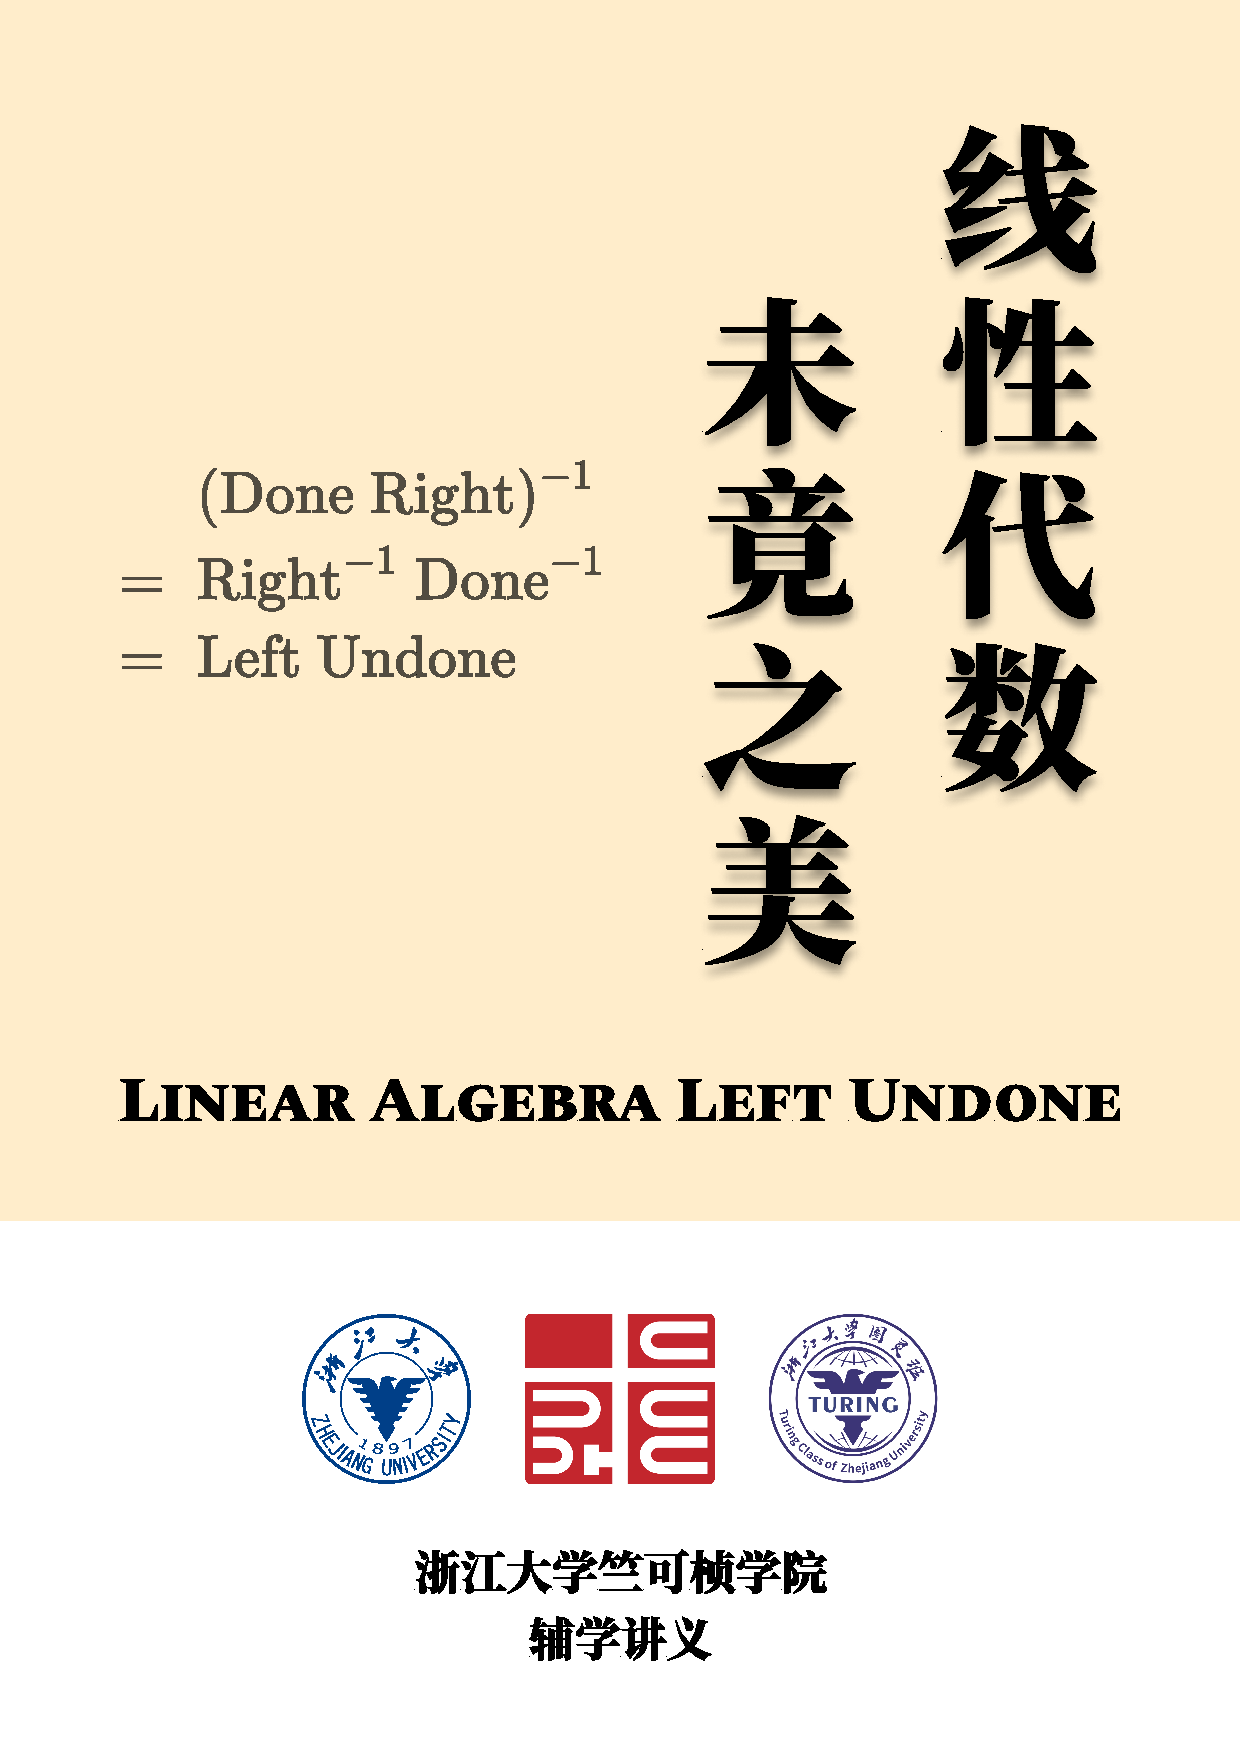
\includepdf[pages={1}]{./figs/cover.pdf}

% \songti

% {% 插入空页
% 	\null
% 	\thispagestyle{empty}
% 	\clearpage
% 	\thispagestyle{empty}
% 	\vspace*{\fill}
\begin{center}
    \Large 致每一个阳光下闪烁着七彩光芒的泡沫

    \vspace{2ex}

    \large \textit{To every bubble glittering with colorful lights under the sun}
\end{center}
\vspace*{\fill}

% }
% \clearpage
% \setcounter{page}{1}
% \chapter*{序}

\section*{一些初衷}

我为这本讲义起了一个大胆的标题,它来源于浙江大学竺可桢学院线性代数II(H)课程选用的教材《线性代数应该这样学》(英文原版名:《Linear Algebra Done Right》)。我们带着半娱乐性质地将最后两个单词像矩阵求逆一样(见封面设计)进行了颠倒,得到了本书的英文名:《Linear Algebra Left Undone》。

接下来我们遇到了一个问题:中文名应该是什么呢?郑俊达同学提供了一个可行解:《线性代数:未竟之美》。转念一想,这一标题不能更契合我们的编写初衷。事实上,我们认为现行的大部分线性代数或高等代数教材具有如下问题,它们也困扰了笔者和许多读者的学习,我们也给出了解决的方案:
\begin{enumerate}
    \item 从线性代数的角度来看,它们的讲解顺序不够自然,大部分教材都从行列式起步,缺乏引入地给出各种概念,使得读者无法理解线性代数的本质。可以说这些教材应当更名``行列式与矩阵计算'',因为线性代数着重研究的线性空间和线性映射反而成为了边缘内容。因此我们采取了更好的讲解思路,更能体现线性代数的美感而非延续高中填鸭式的数学教育——事实上那根本称不上数学,那样的讲授思路根本不够``数学'',失去了数学本身的自然之美,而且使得读者误解数学、厌恶数学;

    \item 浙江大学竺可桢学院两学期线性代数课程选择的《大学数学:代数与几何》和《线性代数应该这样学》教材采用了从抽象空间引入的方式,更贴近本质。但实践过程中许多同学会对``为什么要一开始就学习这些抽象内容''缺乏概念,特别是《线性代数应该这样学》对于工科同学而言``数学味道太浓'',因此最后可能学习效果还不如填鸭式地灌输解题方法。因此我们在讲义中相当于为教材做了很多的注脚,并且优化了整体设计,提供了大量例题习题,都是为了能更自然地引入抽象内容,让读者知道我们为何要学习这些内容,这些内容当年在数学家眼中最自然的状态是什么,这样才能使得抽象的概念易于被初学者接受;

    \item 我们的例题和习题编排也是精心设计过的,不会出现大部分教材使用过程中``上课讲的、作业做的和考试考的脱节''的情况,这一问题不只是很多数学基础课教学的问题,也是国内各个专业都存在的教学问题,笔者也深受其害,所以编写例题习题特别注重对概念和定理的理解、对方法的掌握,不会出现教材中说什么知识很重要但没有例子体会很重要的这种抽象情况,并且大量的习题贴近所学知识也贴近考试,让读者通过习题更好地掌握知识而非反而迷惑不知道自己学了什么,才能更好地体会线性代数的美感而非感受到题海的压迫;

    \item 除了自然的美感外,更重要的是还有``未竟''的美感。线性代数是一个古老而年轻的学科。它发轫于早先对线性方程组的研究,经历了漫长的几何和代数的交错作用,最后又在近世代数的发展过程中被严格化。直到现在,一些相关的内容,例如线性代数群的研究尚且方兴未艾,在现代数学的种种支线当中也有着重要的应用。另外,它的方法论,尤其是其对代数结构的研究在现代数学中也具备着代表性。因此,我们希望呈现一个更广阔的线性代数观,从线性代数出发,对它的现代发展和它在现代数学的各个分支的应用进行一些导论性的介绍,这一方面是为了使得平淡的叙述更加有趣,另一方面也是为了回答一个疑问:线性代数到底有什么用?我们相信,这是许多初学者都有的一个问题,回答这个问题既需要对线性代数的深入学习,也需要有一个现代数学的全局观,这也就带来了本书的另一个部分,未竟专题,也是我们这本书的标题来源。
\end{enumerate}

古人有三不朽:立德、立功、立言,著书立说即为立言。虽说我完全不可能因为编写了一本基础课的讲义而有如此崇高的地位。但在我心里,我已经通过这本讲义将我的热情、我的想法传达给了不少的读者,这样也无愧于我在浙江大学的本科四年。未来或许这本讲义会淹没在历史的风尘中,但我想只要它的某行文字曾经给予读者一丝丝的启发,或更实际地帮助了读者得到了心仪的分数,我想它就是有价值的,我本人的价值也得到了一定的实现。

\section*{本书的面世}

自2021年秋参与浙江大学竺可桢学院学研部(现竺可桢学院学业指导中心)组织的朋辈辅学活动以来,我即将第三次参与线性代数荣誉课的辅学活动。犹记讲义最初的简陋版本,那时为了辅学的期中、期末准备的简单复习提要,里面因为本人时间有限甚至缺少了特征值与特征向量的内容。那时的讲义基本都是知识点的罗列,缺少了许多重要的例题和证明,犹记第一次拿起这个讲义站上讲台的时候,我深刻体会到了这一讲义的不足,因此那次的授课整体而言较为玄学,比较干瘪。因此在2022年再次参加辅学授课时,我借着疫情放开考试延迟的机会分了六个大专题写出了一本相对完整的适合于《大学数学:代数与几何》的复习讲义。里面的讲解比较全面,习题也十分丰富,可以说在复习资料中已经能算过得去的一版了。

但我并不满足于此,我希望这本讲义能成为一本真正的完整的讲义,能兼具配套学习、考试复习的功能,并且在保证体系严谨完整的前提下有更优化的讲解逻辑。因此在2023年的暑假,我基于原先的复习版本进行扩展重排。在这一版本中,我将原先复习资料中的粗略描述都换为了严谨的完整叙述,并且反复打磨讲解顺序,从而更自然地将另一本教材《线性代数应该这样学》的内容自然融合,并且添加了大量的remark更适合于初学者学习。更重要的是,我们中间添加了许多文字叙述,一方面自然引入我们要讲解的内容,这对于初学者而言是很重要的insight,另一方面反复强调我们的行文逻辑,对推进逻辑做适当总结,使得读者能更快地形成体系,同时也补充了很多拓展内容,一些是为了方便读者更自然地理解抽象内容,有一些是契合``未竟之美''的标题,让读者能体会到数学的美感,体会到学习线性代数后我们知识的边界可以推广到多远。

\section*{参考文献}

本讲义作为浙江大学竺可桢学院线性代数荣誉课的辅学讲义,因此核心思路来源于我们选择的教材《大学数学:代数与几何(第二版)》(居余马,李海中)、《大学数学:代数与几何学习辅导》(林翠琴,居余马)、《线性代数应该这样学(第三版)》([美]Sheldon Axler)。

在编写与修订的过程中,我也参考了其他非常多优质的教材或辅导资料,如《高等代数(第二版)》(丘维声)、《高等代数:学习指导书》(丘维声)、《高等代数学(第四版)》(谢启鸿,姚慕生,吴泉水)、《高等代数学(第四版)配套学习用书》(谢启鸿,姚慕生)、《线性代数辅导讲义》(汤家凤)、《高等代数强化讲义》(李扬)以及《高等代数考研:高频真题分类精解300例》等,在复数域的引入部分我也简单参考了王晓光老师的《复变函数讲义(2023版)》,在矩阵计算等专题则部分参考了《数值分析》(Timothy Sauer)、《矩阵分析》(Roger A.Horn,Charles R.Johnson)等计算数学著作。

最后如果读者学完本讲义后对代数学有浓厚的兴趣,非常推荐读者学习后续的抽象代数课程。这里推荐与我同级的图灵班同学编写的\href{https://frightenedfoxcn.github.io/notes/series/alg-for-cs/}{《写给计算机系学生的代数》}作进一步的了解,我们许多高级专题都对这一讲义有引用。

\section*{致谢}

我或许首先需要感谢2022年疫情放开之下的寒冬,没有这学期线性代数考试的延期,我也不会有如此充裕的时间整理出本讲义较为完整的底稿,也就没有这一完整讲义的面世。

我还需要感谢同级的王和钧同学,感谢他当年push我写出了最初版本的复习提要。我要感谢比我低一级的郭苗苗同学,感谢她当年反复邀请我走上讲台实现梦想,虽然可能第一次授课效果一般,但这对于后来我不断打磨授课方式,打磨讲义有非常重要的意义。我也应当感谢竺可桢学院学研部(现竺可桢学院学业指导中心)给我提供了一个辅学的平台,让我通过讲义将我的热情能传达给更多的读者。

我想我也应该特别感谢数学科学学院的吴志祥、谈之奕和刘康生老师,他们在我线性代数入门过程中做了重要的引路人的工作,讲义中许多讲解思路也来源于他们精彩的授课。我也应该特别感谢数学科学学院的王晓光老师,他在复变函数课程以及讲义上的热情以及倾注的心血启发我也应该将我的学习思路和经验通过讲义传达给更多人,并且启发我思考如何从更高的观点、更自然的角度引导读者学习新知识,享受追求真理的过程。

感谢每一位读者和支持者,没有你们的支持,我也不会有如此的热情坚持编写这本讲义,正是有了大家的支持才有了接下来越来越好的版本的面世。特别感谢林前旭同学,他将这本讲义推广到了\href{https://mp.weixin.qq.com/s/nOQ0xzJ0mX2_8JclcKiWdA}{浙江大学微信公众号},这对我而言是极大地鼓舞。

最后,我需要感谢在编写的过程中对本讲义提供了直接的支持的同学:
\begin{itemize}
    \item 梅敏炫同学主编了讲义内积部分;
    \item 高天健同学对线性空间、矩阵、行列式、特征值以及内积等部分提供了宝贵的新讲解思路;
    \item 王普同学主编了线性代数与微积分部分;
    \item 郑俊达同学主编了解析几何部分;
    \item 周健均同学编写了行列式计算进阶以及奇异值分解的应用部分;
    \item 朱熙哲、谢集、郑俊达、郑涵文、李英琦同学负责了答案的初次编写,金政羽、张晋恺、江舜尧、任朱明、赵嘉瑞同学负责了历年卷答案以及正文答案的二次编写;
    \item 王鹤翔同学设计了本讲义的封面;
    \item 李英琦同学全权负责了本讲义的格式设计以及插图;
    \item 刘泓健同学负责了讲义的未竟专题部分。
\end{itemize}
除此之外,还有为我们的\href{https://github.com/yhwu-is/Linear-Algebra-Left-Undone}{GitHub仓库}提出 issue 以及提交 PR 的其他同学。没有他们的支持,这本讲义不会有今天的完整程度。

\begin{flushright}
    \kaishu
    吴一航 \\
    浙江大学计算机科学与技术学院 \\
    \verb|yhwu_is@zju.edu.cn| \\
    2023 年 8 月
\end{flushright}

% \chapter*{致读者}
\addcontentsline{toc}{chapter}{致读者}

\section*{本书特色}
自有底稿成书的念头以来,笔者就十分希望本书能够摆脱市面上大部分线性代数或高等代数教材
固有的一些不够友好的编写风格,力图呈现一本能让读者眼前一亮的讲义。因此本讲义在编写过程
中笔者不断创新讲授思路,大胆摒弃传统的编排风格,总体而言本讲义有如下几大特色:
\begin{enumerate}
    \item 本讲义兼具教材、笔记、复习提纲等多种功能:
    \begin{enumerate}
        \item 说它像是教材,因为我们保留了完整的讲授体系,所有的思路都是反复打磨确认过的,
        保证了整体逻辑的完整和自然;
        \item 说它像是笔记,因为这其中我们特别注重一些细节性的内容,这些内容在教材或授课
        中可能会因为太过平凡被忽略,但在初学中是很重要的,例如我们对求解线性空间像与核、
        求解线性映射矩阵表示的很多讨论都是基于笔者在初学时出现的困惑增添了很多的细节,力求
        读者在初学阶段就能减少因为这些细节带来的困惑;
        \item 说它像是复习提纲,因为在编写过程中我们的很多内容都会分条列出,并且笔者特别
        注意了编写的逻辑连贯性,阅读起来思路比一般教材主线更清晰。除此之外每讲最后还有内容总结,
        并且经常会提供思维导图或是文字描述逻辑等便于读者快速掌握完整的思想体系。
    \end{enumerate}
    \item 本讲义提供了丰富的例题和习题,几乎能覆盖到所有重要的概念、定理和方法,同时
    我们也为这些题目提供了详细的解答,考虑了读者的阅读体验。我们的例题编排特别考虑了初学
    者在学习过程中可能遇到的困难,特别设置了很多适合于加深对概念、定理以及基本方法理解
    的例题。习题我们也是精心挑选,选择难度适中、有助于理解的经典题目,一些技巧性过强
    而脱离线性代数本质的题目我们也会删去或给读者一定的提示。因此我们的讲义特别重视教学和
    习题和考试的一致性,这对于初次学习而言也是非常重要的,也是很多教材没有精心编排而忽略的,
    事实上这会特别影响读者阅读体验;
    \item 在本讲义的编排过程中,我们摒弃了传统的讲授思路。首先我们选择《大学数学:代数与几何》
    以及《线性代数应该这样学》作为参考教材,它们都是从抽象空间出发研究的,相比于一般的线性代数
    或高等代数教材更能深入本质。但我们也考虑到过于抽象的引入对初学者十分不友好,所以我们不断地
    强调我们的讲授逻辑,重视自然地引入概念,自然地推进对概念的研究,最后引申至这些概念对于我们之后
    的研究的重要性。因此编排中我们不断优化内容编排顺序,也添加了足量的补充内容,目的就是使得
    读者能够更自然地接受而非填鸭式地囫囵吞枣,能够真正体会到数学的自然之美而非在抽象的描述或是
    繁杂的技巧中迷失了方向,我想这对于每一个数学学习者而言都是非常关键的。
\end{enumerate}

\section*{阅读建议}
我们为以下四类读者提供如下阅读建议:
\begin{enumerate}
    \item 初学线性代数过程中的读者:那么请坐稳扶好,备好配套的《大学数学:代数与几何》以及
    《线性代数应该这样学》。这本讲义是很好的学习笔记,其中我们有大量的remark帮助读者理解教材中
    可能觉得很平凡的内容,也有大量编排合理的例题和习题帮助读者巩固知识。初学过程中很推荐读者
    阅读我们反复强调的一些逻辑和一些补充的内容从而尽快形成学习体系,这对于数学学习是非常关键的
    ——把握了主线,剩下的就只有一些细节留待补充。当然一些较难的习题不一定在第一次就要掌握,因此
    可以根据自己的接受程度合理选择;
    \item 希望重新学习加深理解的读者:我想这本讲义是非常适合第二次更为深入学习理解的,当然第二次
    学习可以适当略过一些基础和细节内容,但本讲义中很多深入的讨论、独特的思路和有意义的联系一定
    对你第二次学习有所裨益;
    \item 在学习其他方面知识时回顾线性代数基础的读者:无论是基础已经遗忘很多或是还有一定印象的
    读者,本讲义都可以为您提供帮助,因为本书逻辑完整,并且从基础讲起,非常有助于简要回顾一些概念
    帮助后续研究学习其他内容,相比于一些教材填鸭式的讲解更适合于在简短的内容中迅速把握住重点;
    \item 复习考试的读者:如前述本书特色所说,本讲义有大量的通过分点列举总结的内容,每节最后
    也有比较完整的内容总结和逻辑梳理,我们也准备了足量的例题和习题供读者参考。但因为本书是从
    最基础的讲起,并且非常重视一些细节,因此复习时读者可以略过一些过于基础和细节的内容,也可以
    选择性参考讲义中给出的证明等,习题也可以优先选择难度适中的,因为考试中不会出现很难的题目。
\end{enumerate}

\section*{例题与习题}
笔者坚信,没有适量习题练习是很难在初学时较为清晰地掌握线性代数这些抽象的思路以及
运算技巧的,因此本讲义提供了足量的例题与习题便于读者及时巩固学习的概念,并掌握一些
常用的技巧,拓展一些实用的结论,同时一些例题和习题也是讲义完整逻辑中不可或缺的一环。

讲义中的例题有部分是直接概念性的,因为考虑到有一些概念初学时太过抽象,或者一些公式
较为复杂,需要及时联系以熟悉使用.还有一些例题是非常经典的问题,其中的思想在很多其它
习题中都会使用到。基本上在每个重要概念/定理/方法介绍后笔者都会准备合适的例子,并且
都会直接在题目后给出答案。

讲义的习题均设置了A、B、C三组,从低至高区分了难度,读者可以根据自己的实际需求选择
合适难度的习题进行巩固提升。所有的习题都在习题答案分册中提供了解答或思路(教材习题)
可能直接引用),因此读者在思考中遇到困难时可以参考其中的思路,但我们并不推荐直接
参考答案将所有习题粗略过一遍,这样的学习效果十分有限。

\section*{授课建议}
非常欢迎在本讲义的基础上节选或改编出适合辅学授课的讲义,但请注意以下几点:
\begin{enumerate}
    \item 请遵循\href{https://creativecommons.org/licenses/by-nc-sa/4.0/deed.zh}
    {CC BY-NC-SA 4.0}协议,即署名、非商业性使用、相同方式共享;
    \item 本讲义由于笔者本人风格以及目的所在,因此内容较为细致,在授课时您应当有选择性
    地节选内容在课堂上讲授,一些细节性的内容可以在课后让学生自行阅读,否则在有限时间内
    很难讲授较为完整的体系;
    \item 同理,在授课过程中您可以选取对您的授课思路有帮助的经典例题或习题进行讲授。
    授课中题在精不在多,您应当根据自己的授课风格和时间安排合理地选择题目,以有助于
    学生理解以及掌握基本方法为宗旨。
\end{enumerate}

\section*{最后的话}
我们十分清楚,现在阅读这段话的你可能从小到大都对数学缺乏兴趣,也可能在未来与数学之间
不会再有很多的交集。我想很多同学都是经过填鸭式的应试教育而来,如果并非生来热爱,那种
传统的教学方式只能是不断地毁灭式打击学生的数学学习兴趣。

在序言中笔者也提到,这本讲义希望还原数学本原的自然之美,因此从引入到推进到引申,特别是
``未竟之美''部分,我们都尽可能地从自然的角度出发,然后不断深入,让读者能够看到人类目前
研究的模糊边界,能够看到数学的无限魅力。或许从小我们便接受过教育,说数学或许不能帮你买菜,
但其中的``思维方式''才是最重要的。我想,通过本讲义由浅及深的自然推进,读者大概可以体会
当年无数数学家在探索数学本原时的或许``灵光一现''又或许``站在巨人肩膀''背后的思维方式。
更重要的是,这就是追求真理的过程,是一代代数学家用自己有限的生命逼近宇宙无穷,通向崇高
理念世界的过程。我想读者无论是在学习哪个专业,这都是非常重要的精神品质。

尽管我们在编写过程中尽可能地考虑到了读者的阅读体验,但我们也不可能做到面面俱到,
如果内容编排上有什么不合理的地方,或者有什么地方不够清晰,欢迎您将您的阅读体验通过邮件
或直接在本讲义所在的\href{https://github.com/yhwu-is/Linear-Algebra-Left-Undone}
{GitHub仓库}提交issue。如果您希望加入我们的编写团队,将这一讲义传承下去,也欢迎您通过
GitHub仓库提交pull request。

愿诸君热爱数学,热爱对真理的追求。

\begin{flushright}
    \kaishu
    吴一航 \\
    浙江大学计算机科学与技术学院 \\
    yhwu\_is@zju.edu.cn \\
    2023 年 8 月
\end{flushright}

\clearpage
\pdfbookmark[0]{目录}{contents}
\tableofcontents

\addtolength{\parskip}{.5em}

\mainmatter
\setcounter{page}{1} % 将页码计数设置为 1
% 线代I期中/练习
\phantomsection
\section*{2020-2021学年线性代数I(H)小测1}
\addcontentsline{toc}{section}{2020-2021学年线性代数I(H)小测1(谈之奕老师)}

\begin{center}
    任课老师:谈之奕\hspace{4em} 考试时长:90分钟
\end{center}

\begin{enumerate}
	\item[一、](10分)求全部实数$a$,使线性方程组$\begin{cases}
        3x_1+2x_2+x_3=2 \\ x_1-x_2-2x_3=-3 \\ ax_1-2x_2+2x_3=6
    \end{cases}$的解集非空.
	\item[二、](10分)设 $\mathbf{R}^4$ 是 $4$ 维欧氏空间(标准内积),$\alpha=(1,1,1,1),\ \beta=(-1,-1,0,2),\ \gamma=(1,-1,0,0) \in \mathbf{R}^4$,求:
    \begin{enumerate}[label=(\arabic*)]
        \item 与 $\alpha,\ \beta,\ \gamma$ 都正交的一个单位向量 $\delta$;
        \item $||\alpha+\beta+\gamma+\delta||$.
    \end{enumerate}
	\item[三、](15分)记线性映射$\sigma$的核为$\ker\sigma$,像为$\im\sigma$.设$\sigma_1,\sigma_2:V\to V$是线性映射,证明:
	\begin{enumerate}[label=(\arabic*)]
        \item $\ker\sigma_1\subseteq\ker(\sigma_2\circ\sigma_1)$;
        \item $\im(\sigma_2\circ\sigma_1)\subseteq\im\sigma_2$.
    \end{enumerate}
	\item[四、](15分)设$\alpha_1,\alpha_2,\alpha_3$是线性空间$V$的一组基,$T\in\mathcal{L}(V)$,且$T(\alpha_1)=\alpha_1+\alpha_2$,$T(\alpha_2)=\alpha_1-\alpha_2$,$T(\alpha_3)=\alpha_1+2\alpha_2$.求$T$的像空间和核空间,以及$T$的秩.
	\item[五、](15分)设 $W$ 是线性方程组 $\begin{cases}
        x_1-x_2+4x_3-x_4=0 \\ x_1+x_2-2x_3+3x_4=0
    \end{cases}$ 的解空间,求 $W$ 的一组单位正交基,并将其扩充成 $\mathbf{R}^4$ 的单位正交基,这里 $\mathbf{R}$ 是实数域.
	\item[六、](15分)设 $\mathbf{R}[x]_4$ 是数域 $\mathbf{R}$ 上次数小于 $4$ 的多项式所构成的线性空间(约定零多项式次数为 $-\infty$)。$M_2(\mathbf{R})$ 是 $\mathbf{R}$ 上 $2$ 阶方阵所构成的线性空间,定义 $T : \mathbf{R}[x]_4 \to M_2(\mathbf{R})$ 如下,对 $f(x) \in \mathbf{R}[x]_4$,
    \[T(f(x))=\begin{pmatrix}f(0) & f(1) \\ f(-1) & f(0)\end{pmatrix}\]
    \begin{enumerate}
        \item 求出 $T$ 的核空间 $N(T)$ 和像空间 $R(T)$;
        \item 验证关于 $T$ 的维数公式.
    \end{enumerate}
	\item[七、](20分)判断下列命题的真伪,若它是真命题,请给出简单的证明;若它是伪命题,给出理由或举反例将它否定.
	\begin{enumerate}[label=(\arabic*)]
        \item 若$S$是线性空间$V$的线性相关子集,则$S$的每个向量都是$S$的其他向量的线性组合;
        \item 若线性映射$T:V\to W$的核是$K$,则$\dim V=\dim W+\dim K$;
        \item 线性空间$V$的任何子空间$W$都是某个映射$T:V\to V$的核;
        \item 在5维欧式空间$V$中,存在两组线性无关向量$S_1=\{v_1,v_2,v_3\}$和$S_2=\{w_1,w_2,w_3\}$,使其满足内积$\langle v_i,w_j\rangle=0$,其中$i,j=1,2,3$.
    \end{enumerate}
\end{enumerate}

\clearpage

\section*{2020-2021学年线性代数I(H)小测2}
\addcontentsline{toc}{section}{2020-2021学年线性代数I(H)小测2(谈之奕老师)}

\begin{center}
    任课老师:谈之奕\hspace{4em} 考试时长:90分钟
\end{center}

\begin{enumerate}
	\item[一、](10分)称实矩阵$A=(a_{ij})$是整数矩阵,如果每个$a_{ij}$都是整数.设$M$是整数矩阵,且可逆(作为实矩阵).证明:$M$的逆矩阵也是整数矩阵的充要条件是$M$的行列式等于$\pm 1$.
	\item[二、](15分)设$B=\{v_1,v_2,v_3\}$是线性空间$V$的一组基,线性映射$\sigma:V\to V$定义如下:
	\[\sigma(v_1)=v_2+v_3,\sigma(v_2)=v_3,\sigma(v_3)=v_1-v_2.\]
    \begin{enumerate}[label=(\arabic*)]
        \item 求$\sigma$在基$B$下的矩阵;
        \item 证明:$B'=\{v_2,v_3+v_1,v_1-v_2\}$是$V$的另一组基;
        \item 求$\sigma$在基$B'$下的矩阵.
    \end{enumerate}
	\item[三、](15分)设
	\[P=\begin{pmatrix}
        1 & 1 & 0 \\ 0 & 1 & 0 \\ 0 & 0 & 0
    \end{pmatrix},\enspace Q=\begin{pmatrix}
        0 & 0 \\ 1 & 0
    \end{pmatrix},\]
    定义$\mathbf{R}^{3\times 2}$上映射$\sigma$:
    \[\sigma(A)=PAQ.\]
    \begin{enumerate}[label=(\arabic*)]
        \item 验证$\sigma$是线性映射;
        \item 求$\im\sigma$和$\ker\sigma$;
        \item 验证关于$\sigma$的维数公式.
    \end{enumerate}
	\item[四、](15分)求参数 $a,\ b$  的值,使得 $\begin{vmatrix}1 & 1 & 1 \\ x & y & z \\u & v & w\end{vmatrix}=1,\ \begin{vmatrix}1 & 2 & -5 \\ x & y & z \\u & v & w\end{vmatrix}=2,\ \begin{vmatrix}2 & 3 & b \\ x & y & z \\u & v & w\end{vmatrix}=a$ 都成立,并求$\begin{vmatrix}x & y & z \\ 1 & -1 & 5 \\u & v & w\end{vmatrix}$.
	\item[五、](15分)设在$\mathbf{F}[x]_3$中有两组基:
	\[(A)\alpha_1=1-x,\alpha_2=-x+x^2,\alpha_3=3x-2x^2;\]
    \[(B)\beta_1=4x+5x^2,\beta_2=-1,\beta_3=3x+4x^2.\]
    \begin{enumerate}[label=(\arabic*)]
        \item 求基$(A)$到基$(B)$的过渡矩阵;
        \item 设$\alpha$在基$(A)$下的坐标为$(1,1,-1)^{\mathrm{T}}$,求$\alpha$在基$(B)$下的坐标.
    \end{enumerate}
	\item[六、](10分)设 $A \in M_{m \times n}(\mathbf{F})$,$r(A)=r$,$k$ 是满足条件 $r \leq k \leq n$ 的任意整数,证明存在 $n$ 阶方阵 $B$,使得 $AB=0$,且 $r(A)+r(B)=k$.
	\item[七、](20分)判断下列命题的真伪,若它是真命题,请给出简单的证明;若它是伪命题,给出理由或举反例将它否定.
	\begin{enumerate}[label=(\arabic*)]
        \item 域$\mathbf{F}$上的全体$n$阶可逆矩阵构成$M_n(\mathbf{F})$的一个子空间;
        \item 设$A$和$B$都是可逆矩阵,则矩阵$\begin{pmatrix}
            O & B \\ A & C
        \end{pmatrix}$也是可逆矩阵;
        \item 可逆矩阵$A$的伴随矩阵$A^*$的行列式等于1;
        \item 若对于任何正整数$n$,方阵$A$(阶数大于1)的$n$次乘积$A^n$都是非零方阵,则$A$可逆.
    \end{enumerate}
\end{enumerate}

\clearpage

\phantomsection
\section*{2020-2021学年线性代数I(H)期中}
\addcontentsline{toc}{section}{2020-2021学年线性代数I(H)期中(吴志祥老师)}

\begin{center}
    任课老师:吴志祥\hspace{4em} 考试时长:120分钟
\end{center}
\begin{enumerate}
	\item[一、](10分)设方程组:
    \[\begin{cases}
        x_1-x_2+x_3-x_4=0 \\ 2x_1+4x_2-5x_3+7x_4=0\\ax_1+3x_2-4x_3+6x_4=0
    \end{cases}\]
    的解空间为 $V_1$,方程组:
    \[\begin{cases}
        4x_1+2x_2-3x_3+bx_4=0 \\ 5x_1+7x_2-9x_3+13x_4=0\\3x_1-3x_2+3x_3-2x_4=0
    \end{cases}\]

    的解空间为 $V_2$ ,问 $a,b$ 为何值时,$\mathbf{R}^4=V_1 \oplus V_2$.
	\item[二、](10分)设 $V=\{(a_{ij})_{n \times n}\ |\ \forall i,\ j,\ a_{ij}=a_{ji}\}$
    \begin{enumerate}[label=(\arabic*)]
        \item 证明:$V$ 为 $F^{n \times n}$ 的子空间;

        \item 求 $V$ 的基和维数.
    \end{enumerate}
	\item[三、](10分)设 $f_1=-1+x,\ f_2=1-x^2,\ f_3=1-x^3,\ g_1=x-x^2,\ g_2=x+x^3,\ V_1=L\left(f_1,\ f_2,\ f_3\right),\ V_2=L\left(g_1,\ g_2\right)$,求:
    \begin{enumerate}[label=(\arabic*)]
        \item $V_1+V_2$ 的基和维数;

        \item $V_1 \cap V_2$ 的基和维数;

        \item $V_2$ 在 $\mathbf{R}[x]_4$ 空间的补.
    \end{enumerate}
	\item[四、](10分)设 $\epsilon_1,\ \epsilon_2$ 为 $n$ 维欧氏空间 $V$ 的两个单位正交向量,定义
    \[\sigma(\alpha)=\alpha-2(\alpha,\epsilon_1)\epsilon_1-2(\alpha,\epsilon_2)\epsilon_2\]
    证明:
    \begin{enumerate}
        \item $\sigma$ 是 $V$ 上的线性变换;

        \item $\forall \alpha,\ \beta \in V,\ \left(\sigma (\alpha),\sigma (\beta) \right)=\left(\alpha,\beta\right)$.
    \end{enumerate}
	\item[五、](10分)已知 $n$ 阶矩阵 $A$ 的秩为 1 ,证明:$A^k=\textup{tr}(A)^{k-1}A$.(注:$\textup{tr}$ 为矩阵的迹,即矩阵的对角线元素之和)
	\item[六、] (10分)已知矩阵 $A=\begin{pmatrix}a & b & c \\ d & e & f \\ h & x & y\end{pmatrix}$ 的逆是 $A^{-1}=\begin{pmatrix}-1 & -2 & -1 \\ 2 & 1 & 0 \\ 0 & -3 & -1\end{pmatrix}$,且已知矩阵$B=\begin{pmatrix}a-2b & b-3c & -c \\ d-2e & e-3f & -f \\ h-2x & x-3y & -y\end{pmatrix}$. 求矩阵 $X$ 满足:
    \[X+(B(A^\mathrm{T}B^2)^{-1}A^\mathrm{T})^{-1}=X(A^2(B^\mathrm{T}A)^{-1}B^\mathrm{T})^{-1}(A+B).\]
	\item[七、](10分)设 $V(\mathbf{F})$ 是一个 $n$ 维线性空间,$\sigma \in L(V,V)$,证明:
    \begin{enumerate}[label=(\arabic*)]
        \item 在 $\mathbf{F}[x]$ 中有一个次数不高于 $n^2$ 的多项式 $p(x)$ 使 $p(\sigma)=0$;

        \item $\sigma$ 可逆$\iff$有一常数项不为 0 的多项式 $p(x)$ 使 $p(\sigma)=0$.
    \end{enumerate}

\item[八、](10分)已知三维线性空间 $V$ 的线性变换 $\sigma$ 关于基 $\{\alpha_1,\alpha_2,\alpha_3\}$ 所对应的矩阵为
    \[\begin{pmatrix}1 & 2 & -1 \\ 2 & 1 & 0 \\ 3 & 0 & 1\end{pmatrix}\]
    \begin{enumerate}[label=(\arabic*)]
        \item 求 $\sigma$ 在基 $\{\beta_1,\ \beta_2,\ \beta_3\}$ 下对应的矩阵 $B$,其中:
        \[\beta_1=2\alpha_1+\alpha_2+3\alpha_3,\ \beta_2=\alpha_1+\alpha_2+2\alpha_3,\ \beta_3=-\alpha_1+\alpha_2+\alpha_3\]

        \item 求 $\sigma$ 的值域 $\sigma(V)$ 和核 $\textup{ker}\sigma$;

        \item 把 $\sigma(V)$ 的基扩充为 $V$ 的基,并求 $\sigma$ 在这组基下对应的矩阵;

        \item 把 $\textup{ker}\sigma$ 的基扩充为 $V$ 的基,并求 $\sigma$ 在这组基下对应的矩阵.
    \end{enumerate}
	\item[九、](20分)判断下列命题的真伪,若它是真命题,请给出简单的证明;若它是伪命题,给出理由或举反例将它否定.
    \begin{enumerate}[label=(\arabic*)]
        \item 若 $\alpha_1,\ \alpha_2,\ \alpha_3$ 线性相关,则 $\alpha_1+\alpha_2,\ \alpha_2+\alpha_3,\ \alpha_3+\alpha_1$ 也线性相关;

        \item 一个有限维线性空间只包含有限个子空间;

        \item 已知 $\sigma \in L(V,\ V)$,$\textup{dim}V=n$,则由 $r(\sigma)+\textup{dim(ker}\sigma)=n$ 可得$\textup{Im}\sigma+\textup{ker}\sigma=V$;

        \item 若对于任何正整数 $n$,方阵 $A$ ( 阶数大于 1 ) 的 $n$ 次乘积 $A^n$ 都是非零方阵,则 $A$ 是可逆的.
    \end{enumerate}
\end{enumerate}

\clearpage

\phantomsection
\section*{2021-2022学年线性代数I(H)小测}
\addcontentsline{toc}{section}{2020-2021学年线性代数I(H)小测(刘康生老师)}

\begin{center}
    任课老师:刘康生\hspace{4em} 考试时长:90分钟
\end{center}
\begin{enumerate}
	\item[一、] 设矩阵$A=\begin{pmatrix}
        a & -1 & 1 \\ -1 & a & -1 \\ 1 & -1 & a
    \end{pmatrix}$,$\beta=\begin{pmatrix}
        0 \\ 1 \\ 1
    \end{pmatrix}$. 假设线性方程组$Ax=\beta$有解但解不唯一.
    \begin{enumerate}[label=(\arabic*)]
        \item 求$a$的值;

        \item 给出$Ax=\beta$的一般解.
    \end{enumerate}
	\item[二、]设
	\[P=\begin{pmatrix}
        1 & 1 & 0 \\ 0 & 1 & 0 \\ 0 & 0 & 0
    \end{pmatrix},\enspace Q=\begin{pmatrix}
        0 & 0 \\ 1 & 0
    \end{pmatrix},\]
    定义$\mathbf{R}^{3\times 2}$上映射$\sigma$:
    \[\sigma(A)=PAQ.\]
    \begin{enumerate}[label=(\arabic*)]
        \item 验证$\sigma$是线性映射;

        \item 求$\im\sigma$和$\ker\sigma$;

        \item 验证关于$\sigma$的维数公式.
    \end{enumerate}
	\item[三、]设$B$是$3\times 1$矩阵,$C$是$1\times 3$矩阵,证明:$r(BC)\leqslant 1$;反之,若$A$是秩为1的$3\times 3$矩阵,证明:存在$3\times 1$矩阵$B$和$1\times 3$矩阵$C$,使得$A=BC$.
	\item[四、]设$B=\{\beta_1,\beta_2,\ldots,\beta_n\}$是实数域$\mathbf{R}$上线性空间$V$的一组基,$T\in\mathcal{L}(V)$,$T(\beta_1)=\beta_2$,$T(\beta_2)=\beta_3$,$\cdots$,$T(\beta_{n-1})=\beta_n$,$T(\beta_n)=\sum\limits_{i=1}^{n}a_i\beta_i(a_i\in\mathbf{R})$. 求$T$在$B$下的表示矩阵. 在什么条件下$T$是同构映射?
	\item[五、]设$A^*$是$n$阶方阵$A$的伴随矩阵,求$A^*$的秩.
	\item[六、]判断下列命题的真伪,若它是真命题,请给出简单的证明;若它是伪命题,给出理由或举反例将它否定.
	\begin{enumerate}[label=(\arabic*)]
        \item 给定线性空间$V$的非零向量$v$和线性空间$W$的向量$w$,总存在线性映射$T:V\to W$,使得$T(v)=w$;

        \item 若线性方程组有$m$个方程,$n$个变量,且$m<n$,则这个方程组一定有非零解;

        \item 若方阵$A^3=0$,则$E+A$和$E-A$都是可逆矩阵;

        \item 若方阵$A^2=A$,则$E+A$和$E-A$都是可逆矩阵.
    \end{enumerate}
\end{enumerate}

\clearpage

\section*{2021-2022学年线性代数I(H)期中}
\addcontentsline{toc}{section}{2021-2022学年线性代数I(H)期中(吴志祥老师)}

\newpage

\section*{2022-2023学年线性代数I(H)期中}
\addcontentsline{toc}{section}{2022-2023学年线性代数I(H)期中(刘康生老师)}

\begin{center}
    任课老师:刘康生\hspace{4em} 考试时长:45分钟
\end{center}
\begin{enumerate}
	\item[一、] 设矩阵$A=\begin{pmatrix}
        a & -1 & 1 \\ -1 & a & -1 \\ 1 & -1 & a
    \end{pmatrix}$,$\beta=\begin{pmatrix}
        0 \\ 1 \\ 1
    \end{pmatrix}$.假设线性方程组$Ax=\beta$有解但解不唯一.
    \begin{enumerate}[label=(\arabic*)]
        \item 求$a$的值;
        \item 给出$Ax=\beta$的所有解.
    \end{enumerate}
	\item[二、]设
	\[P=\begin{pmatrix}
        1 & 1 & 0 \\ 0 & 1 & 0 \\ 0 & 0 & 0
    \end{pmatrix},\enspace Q=\begin{pmatrix}
        0 & 0 \\ 1 & 0
    \end{pmatrix},\]
    定义$\mathbf{R}^{3\times 2}$上映射$\sigma$:
    \[\sigma(A)=PAQ.\]
    \begin{enumerate}[label=(\arabic*)]
        \item 验证$\sigma$是线性映射;
        \item 求$\im\sigma$和$\ker\sigma$;
        \item 求$\mathbf{R}^{3\times 2}$的两组基$B_1,B_2$,使得$\sigma$在$B_1,B_2$下的矩阵为对角矩阵.
    \end{enumerate}
	\item[三、]设$B=\{\beta_1,\beta_2,\cdots,\beta_n\}$是实数域$\mathbf{R}$上线性空间$V$的一组基,$T\in\mathcal{L}(V)$,$T(\beta_1)=\beta_2$,$T(\beta_2)=\beta_3$,$\cdots$,$T(\beta_{n-1})=\beta_n$,$T(\beta_n)=\sum\limits_{i=1}^{n}a_i\beta_i(a_i\in\mathbf{R})$.求$T$在$B$下的表示矩阵.在什么条件下$T$是同构映射?
	\item[四、]判断下列命题的真伪,若它是真命题,请给出简单的证明;若它是伪命题,给出理由或举反例将它否定.
	\begin{enumerate}[label=(\arabic*)]
        \item 若$W$是线性空间$V$的子空间,$\alpha\in V$,则$\alpha+W$是$V$的子空间;
        \item 若$W$是线性空间$V$的子空间,对任何的$\alpha\in V$,定义$\overline{\alpha}=\alpha+W$,则
        \[\overline{\alpha}=\overline{\beta}\text{ 或者 }\overline{\alpha}\cap\overline{\beta}=\varnothing;\]
        \item 若方阵$A^3=0$,则$E+A$和$E-A$都是可逆矩阵;
        \item 若方阵$A^2=A$,则$E+A$和$E-A$都是可逆矩阵.
    \end{enumerate}
\end{enumerate}

\clearpage

\section*{2022-2023学年线性代数I(H)期中}
\addcontentsline{toc}{section}{2022-2023学年线性代数I(H)期中(谈之奕老师)}

\begin{center}
    任课老师:谈之奕\hspace{4em} 考试时长:90分钟
\end{center}
\begin{enumerate}
	\item[一、](15分)参数$\lambda$取何值时,线性方程组
	\[\begin{cases}
        2x_1-4x_2+5x_3+3x_4=1 \\
        3x_1-6x_2+4x_3+2x_4=2 \\
        4x_1-8x_2+3x_3+x_4=\lambda
    \end{cases}\]
    有解?当方程组有解时,求其一般解.
	\item[二、](15分)设$\alpha_1=(1,1,1,2)^\mathrm{T}$,$\alpha_2=(3,4,4,7)^\mathrm{T}$,$\alpha_3=(-2,1,2,-3)^\mathrm{T}$,$\alpha_4=(5,3,4,6)^\mathrm{T}$,$\alpha_5=(4,5,3,13)^\mathrm{T}$,试求向量组$\{\alpha_1,\alpha_2,\alpha_3,\alpha_4,\alpha_5\}$的一组极大线性无关组.
	\item[三、](15分)
    \begin{enumerate}[label=(\arabic*)]
        \item 已知$\mathbf{R}^2$上的线性变换$\sigma(x_1,x_2)=(x_1-x_2,2x_1-2x_2)$,$I$为$\mathbf{R}^2$上的恒等变换,求$\ker\sigma$和$\im(I-\sigma)$;
        \item 设$\tau$为$\mathbf{R}^n$上任一线性变换,$I$为$\mathbf{R}^n$上恒等变换,证明:$\ker\tau\subseteq\im(I-\tau)$.又$\im\tau\subseteq\ker(I-\tau)$是否一定成立?
    \end{enumerate}
	\item[四、](25分)设$\mathbf{R}[x]_3$是次数小于等于3的实系数多项式的全体和零多项式一起组成的集合关于多项式加法和数乘构成的实数域上的线性空间.
	\begin{enumerate}[label=(\arabic*)]
        \item 证明:$W=\{f(x)\in\mathbf{R}[x]_3\mid f(1)=0\}$是$\mathbf{R}[x]_3$的子空间,并求$\dim W$和$W$的一组基;
        \item 定义从$\mathbf{R}[x]_3$到$\mathbf{R}$的映射$T$如下:对任意$f(x)\in\mathbf{R}[x]_3$,$T(f(x))=f(1)$,证明:$T$是线性映射,并求$\dim\ker T$和$\im T$;
        \item 设$f,g,h\in\mathbf{R}[x]_3$,且$f(1)=g(1)=h(1)=0$,证明:$f,g,h$线性相关.
    \end{enumerate}
	\item[五、](30分)判断下列命题的真伪,若它是真命题,请给出简单的证明;若它是伪命题,给出理由或举反例将它否定.
    \begin{enumerate}[label=(\arabic*)]
        \item 向量$\beta$不能由向量组$\alpha_1,\cdots,\alpha_n$线性表示,则向量组$\alpha_1,\cdots,\alpha_n,\beta$线性无关;
        \item 实数集$\mathbf{R}$对实数的加法与实数的乘法构成任意数域上的线性空间;
        \item 记$\mathbf{R}_k^n$为至多有$k$个分量为非零实数的$n$元向量全体,$\mathbf{R}_k^n$是$\mathbf{R}^n$的子空间;
        \item 若$S$是线性空间$V$的线性相关子集,则$S$的每个向量都是$S$的其他向量的线性组合;
        \item 若线性映射$T:V\to W$的核是$K$,则$\dim V=\dim W+\dim K$;
        \item 线性空间$V$的任何子空间$W$都是某个映射$T:V\to V$的核.
    \end{enumerate}
\end{enumerate}

\clearpage

\phantomsection
\section*{2022-2023学年线性代数I(H)期中}
\addcontentsline{toc}{section}{2022-2023学年线性代数I(H)期中(吴志祥老师)}

\begin{center}
    任课老师:吴志祥\hspace{4em} 考试时长:90分钟
\end{center}

\begin{enumerate}
	\item[一、](10分)讨论当$a$取何值时,下列方程组有解?无解?
	\[\begin{cases}
        x_1+x_2+x_3+x_4+x_5=1 \\
        3x_1+2x_2+x_3+x_4-3x_5=a \\
        x_2+2x_3+2x_4+6x_5=3 \\
        5x_1+4x_2+3x_3+3x_4-x_5=2
    \end{cases}.\]
	\item[二、](10分)证明向量组$\{2\alpha_1+\alpha_2,2\alpha_2+\alpha_3,2\alpha_3+\alpha_1\}$线性无关的充分必要条件是向量组$\{\alpha_1,\alpha_2,\alpha_3\}$线性无关.
	\item[三、](10分)已知向量$\alpha_1=(1,2,4,3)^\mathrm{T},\enspace \alpha_2=(1,-1,-6,6)^\mathrm{T},\enspace \alpha_3=(-2,-1,2,-9)^\mathrm{T},\enspace \alpha_4=(1,1,-2,7)^\mathrm{T},\enspace \beta=(4,2,4,a)^\mathrm{T}$.
    \begin{enumerate}[label=(\arabic*)]
        \item 求子空间$W=\spa(\alpha_1,\alpha_2,\alpha_3,\alpha_4)$的维数和一组基;

        \item 求$a$的值,使得$\beta\in W$,并求$\beta$在(1)中选取的基下的坐标.
    \end{enumerate}
	\item[四、](10分)设$\{\varepsilon_1,\varepsilon_2,\varepsilon_3,\varepsilon_4\}$是欧式空间$V$的一组标准正交基,$W=\spa(\alpha_1,\alpha_2,\alpha_3)$,其中$\alpha_1=\varepsilon_1+\varepsilon_2+\varepsilon_3+\varepsilon_4,\alpha_2=3\varepsilon_1+3\varepsilon_2-\varepsilon3-\varepsilon_4,\alpha_3=-2\varepsilon_1+6\varepsilon_3+8\varepsilon_4$.
	\begin{enumerate}[label=(\arabic*)]
        \item 求$\alpha_1,\alpha_2$的夹角;

        \item 求$W$的一组标准正交基.
    \end{enumerate}
	\item[五、](10分)已知$f_1=1-x,f_2=1+x^2,f_3=x+2x^2$是$\mathbf{R}[x]_3$中三个元素,$\sigma$是$\mathbf{R}[x]_3$上的线性变换且满足$\sigma(f_1)=2+x^2,\sigma(f_2)=x,\sigma(f_3)=1+x+x^2$.
    \begin{enumerate}[label=(\arabic*)]
        \item 证明:$f_1,f_2,f_3$构成$\mathbf{R}[x]_3$的一组基;

        \item 求$\sigma$在基$\{f_1,f_2,f_3\}$下的矩阵;

        \item 设$f=1+2x+3x^2$,求$\sigma(f)$.
    \end{enumerate}
	\item[六、](10分)已知$\mathbf{R}^3$的两个线性变换$\sigma,\tau$为
	\[\sigma(x_1,x_2,x_3)=(x_1+2x_2+3x_3,-x_1+2x_2-x_3,0),\]
    \[\tau(x_1,x_2,x_3)=(x_2,x_3,0).\]
    \begin{enumerate}[label=(\arabic*)]
        \item 求$r(\sigma+\tau)$和$r(\sigma\tau)$;

        \item 求$\im\sigma+\ker\sigma$.
    \end{enumerate}
	\item[七、](10分)设$M_n(\mathbf{R})$是实数域$\mathbf{R}$上所有$n$阶矩阵组成的集合. 设$W=\{A\in M_n(\mathbf{R})\mid a_{ji}=ka_{ij},\enspace i\leqslant j\}$,求当$k=0,1,2$时,$W$的一组基和维数.

    \item[八、](10分)设$V$是域$\mathbf{F}$上的$n$维线性空间,$\alpha_1,\alpha_2,\ldots,\alpha_n$是$V$的一组基,且
    \begin{gather*}
        V_1=\spa(\alpha_1+2\alpha_2+\cdots+n\alpha_n) \\
        V_2=\left\{k_1\alpha_1+k_2\alpha_2+\cdots+k_n\alpha_n \;\middle|\; k_1+\dfrac{k_2}{2}+\cdots+\dfrac{k_n}{n}=0\right\}
    \end{gather*}
    证明:
    \begin{enumerate}[label=(\arabic*)]
        \item $V_2$是$V$的子空间;

        \item $V=V_1\oplus V_2$.
    \end{enumerate}
	\item[九、](20分)判断下列命题的真伪,若它是真命题,请给出简单的证明;若它是伪命题,给出理由或举反例将它否定.
    \begin{enumerate}[label=(\arabic*)]
        \item $\forall n\geqslant 2$,不存在非零实线性映射$f:M_n(\mathbf{R})\to\mathbf{R}$使得$f(AB)=f(A)f(B)$;

        \item 设$W_1,W_2$是线性空间$V$的两个子空间,$W_1\cup W_2=W_1+W_2$当且仅当$W_1\subseteq W_2$或$W_2\subseteq W_1$;

        \item 设$\alpha,\beta$是欧式空间$V$中两个线性无关向量,且$\cfrac{2(\alpha,\beta)}{(\alpha,\alpha)}$和$\cfrac{2(\alpha,\beta)}{(\beta,\beta)}$都是不大于零的整数,则$\alpha$和$\beta$的夹角只可能是$\cfrac{\pi}{2}$,$\cfrac{2\pi}{3}$,$\cfrac{3\pi}{4}$,$\cfrac{5\pi}{6}$;

        \item $n$是一个大于1的整数,$W=\{(x_1,x_2,\ldots,x_n)\in\mathbf{C}^n\mid x_1^2+x_2^2+\cdots+x_n^2=0\}$是复线性空间$\mathbf{C}^n$的一个子空间.
    \end{enumerate}
\end{enumerate}

\clearpage


% 线代I期末
\phantomsection
\section*{2009-2010学年线性代数I(H)期末}
\addcontentsline{toc}{section}{2009-2010学年线性代数I(H)期末}

\begin{center}
    任课老师:统一命卷\hspace{4em} 考试时长:120分钟
\end{center}

\begin{enumerate}
    \item [一、](10分)记 $C([0,2\pi],\mathbf{R})$ 是区间 $[0,2\pi]$ 上全体连续函数作成的实线性空间,对 $f,g \in C([0,2\pi],\mathbf{R})$,用
    \[(f,g) = \displaystyle\int_0^{2\pi}f(x)g(x)\mathrm{d}x\]
    来定义内积. 如果
    \[f,g:[0,2\pi] \to \mathbf{R},f(x)=x,g(x)=\sin x\]
    求 $f$ 与 $g$ 的夹角 $\theta$.

    \item[二、](10分)设 $V$ 是次数 $\leqslant 2$ 的实多项式线性空间,$T:V\to V$,
    \[T(f(x)) = f(x) + xf'(x).\]
    求 $T$ 的特征值. 对于每个特征值,求属于它的特征子空间.

    \item[三、](10分)设 $B$ 是 $3\times 1$ 矩阵,$C$ 是 $1\times 3$ 矩阵,证明:$r(BC)\leqslant 1$;反之,若 $A$ 是秩为 1的 $3\times 3$ 矩阵,证明:存在 $3\times 1$ 矩阵 $B$ 和 $1\times 3$ 矩阵 $C$,使得 $A=BC$.

    \item[四、](10分)设矩阵 $A=\begin{pmatrix}a & -1 & 1 \\ -1 & a & -1 \\ 1 & -1 & a\end{pmatrix},\beta =\begin{pmatrix}0 \\ 1 \\ 1\end{pmatrix}$. 假设线性方程组 $AX=\beta$ 有解但解不唯一.
    \begin{enumerate}[label=(\arabic*)]
        \item 求 $a$ 的值;

        \item 给出 $AX=\beta$ 的一般解.
    \end{enumerate}

\item[五、](10分)设 $A$ 是可逆实矩阵.
    \begin{enumerate}[label=(\arabic*)]
        \item 证明 $A^{\mathrm{T}}A$ 是对称矩阵;

        \item 证明 $A^{\mathrm{T}}A$ 是正定的.
    \end{enumerate}

\item[六、](10分)令 $A = \begin{pmatrix}0 & 1 & 1 \\ 1 & -2 & 2 \\ 1 & 2 & -1 \end{pmatrix} \in M_{3\times 3}(\mathbf R)$.
    \begin{enumerate}[label=(\arabic*)]
        \item 求可逆矩阵 $Q\in M_{3\times 3}(\mathbf R)$ 使 $Q^{\mathrm{T}}AQ$ 是对角矩阵;

        \item 给出 $A$ 的正惯性指数、负惯性指数,并确定 $A$ 的定性.
    \end{enumerate}

\item[七、](10分)设 $\beta=\{v_1,v_2,\ldots,v_n\}$ 是 $V$ 的一组基,$T:V\to V$ 是线性变换,

    $T(v_1)=v_2,T(v_2)=v_3,\ldots,T(v_{n-1})=v_n,T(v_n)=a_1v_1+a_2v_2+\cdots+a_nv_n$.

    求 $T$ 关于 $\beta$ 的矩阵表示. 以及,在什么条件下 $T$ 是同构?

    \item[八、](10分)设 $A\in M_{n\times n}(\mathbf{F})$ 有两个不同的特征值 $\lambda_1,\lambda_2$,且属于 $\lambda_1$ 的特征子空间的维数是$n-1$,证明:$A$ 是可对角化的.

    \item[九、](20分)判断下面命题的真伪. 若它是真命题,给出一个简单证明;若它是伪命题,举一个具体的反例将它否定.
    \begin{enumerate}[label=(\arabic*)]
        \item 给定线性空间 $V$ 的非零向量 $v$ 和线性空间 $W$ 的向量 $w$,总存在线性映射 $T:V\to W$ 使得 $T(v)=w$.

        \item 若线性方程组有 $m$ 个方程,$n$ 个变量,且 $m < n$,则这个方程组一定有非零解.

        \item 若 $n$ 阶方阵 $A$ 的秩是 $n$,则 $A$ 是可逆的.

        \item 正交变换是可对角化的.
    \end{enumerate}
\end{enumerate}

\clearpage

\phantomsection
\section*{2010-2011学年线性代数I(H)期末}
\addcontentsline{toc}{section}{2010-2011学年线性代数I(H)期末}

\begin{center}
    任课老师:统一命卷\hspace{4em} 考试时长:120分钟
\end{center}

\begin{enumerate}
    \item [一、](10分)求全部的实数 $a$,使线性方程组$\begin{cases} 3x_1+2x_2+x_3=2 \\ x_1-x_2-2x_3=-3 \\ ax_1-2x_2+2x_3 = 6\end{cases}$ 的解集非空.

    \item [二、](10分)设 $M_{3\times2} (\mathbf{F})$ 是数域 $\mathbf{F}$ 上全体 $3\times 2$ 矩阵构成的线性空间,
    \[P = \begin{pmatrix}1 & 1 & 0 \\ 0 & 1 & 0 \\ 0 & 0 & 0\end{pmatrix},Q=\begin{pmatrix}0 & 0 \\ 1 & 0\end{pmatrix}.\]
    定义 $T:M_{3\times 2}(\mathbf{F}) \to M_{3\times2} (\mathbf{F})$ 如下,对任意的 $A\in M_{3\times2}(\mathbf{F})$ 有 $T(A) = PAQ$.
    \begin{enumerate}[label=(\arabic*)]
        \item 证明 $T$ 是线性映射.

        \item 求出 $T$ 的像空间和核空间.

        \item 验证关于 $T$ 的维数公式.
    \end{enumerate}

\item [三、](10分)设 $A$ 和 $B$ 是 $n$ 阶方阵,其中 $n$ 是奇数. 若 $AB=-BA$,证明:$A$ 是不可逆的或者 $B$ 是不可逆的.

    \item [四、](10分)设 $V$ 是欧氏空间, $\mathbf{u,v}\in V$ 且 $\mathbf{v} \neq \mathbf{0}$.  证明
    \[\lvert(\mathbf{u,v}) \rvert =\lvert \mathbf{u} \rvert \lvert \mathbf{v} \rvert \]
    当且仅当存在 $\lambda \in \mathbf{R}$,使 $\mathbf{u} = \lambda \mathbf{v}$.

    \item [五、](10分)设 $A=(a_{ij})_{n\times n}$ 是实正交矩阵.
    \begin{enumerate}[label=(\arabic*)]
        \item 证明 $\lvert\sum\limits_{i=1}^n{a_{ii}}\rvert \leqslant n$.

        \item 在什么条件下等式成立?
    \end{enumerate}

\item [六、](10分)求 $2\times 2$ 实矩阵 $A$,使得 $A$ 的特征值是 2 和 1,而对应于 2 的特征子空间由 $\begin{pmatrix}1 \\ 1\end{pmatrix}$生成,对应于 1 的特征子空间由 $\begin{pmatrix}2 \\ 1\end{pmatrix}$ 生成.

    \item [七、](10分)设 $n$ 阶方阵 $A$ 和 $B$ 都可对角化,并且它们有相同的特征子空间(但不一定有相同的特征值),证明 $AB=BA$.

    \item [八、](10分)实三元二次多项式 $f:\mathbf{R^3}\to \mathbf{R}$ 的定义是
    \[f(x,y,z) = 2x^2-8xy+y^2-16xz+14yz+5z^2.\]
    \begin{enumerate}[label=(\arabic*)]
        \item 给出 $3\times 3$ 实对称矩阵 $A$,使 $f(x,y,z) = (x,y,z)A(x,y,z)^{\mathbf{T}}$.

        \item 给出一个与 $A$ 相合的对角矩阵.

        \item 给出 $A$ 的秩,正惯性指数和负惯性指数.
    \end{enumerate}

\item [九、](20分)判断下面命题的真伪. 若它是真命题,给出一个简单证明;若它是伪命题,举一个具体的反例将它否定.
    \begin{enumerate}[label=(\arabic*)]
        \item 若线性映射 $T_1,T_2:V \to W$ 对 $V$ 的一组基中的每一个基向量 $v$ 满足 $T_1(v)=T_2(v)$,则 $T_1=T_2$.

        \item 若对于任何正整数 $n$,方阵 $A$(阶数大于 1)的 $n$次乘积 $A^n$ 都是非零方阵,则 $A$ 可逆.

        \item 若线性映射 $T:V\to W$ 的核是 $K$,则 $\mathrm{dim}V=\mathrm{dim}W+\mathrm{dim}K$.

        \item 若方阵 $A$ 相似于方阵 $B$,则 $A$ 与 $B$ 有相同的特征向量.
    \end{enumerate}
\end{enumerate}

\clearpage

\section*{2011-2012学年线性代数I(H)期末}
\addcontentsline{toc}{section}{2011-2012学年线性代数I(H)期末}

\newpage

\section*{2012-2013学年线性代数I(H)期末}
\addcontentsline{toc}{section}{2012-2013学年线性代数I(H)期末}

\begin{center}
    任课老师:统一命卷\hspace{4em} 考试时长:120分钟
\end{center}

\begin{enumerate}
    \item [一、](10分)求实线性方程组 $\begin{cases}x_1-x_2+2x_3 = 1 \\ x_1-2x_2-x_3=2 \\ 3x_1-x_2+5x_3=3 \\ 2x_1-2x_2-3x_3 = 4\end{cases}$ 的解集.
    \item [二、](10分)设 $A$ 是域 $\mathbf{F}$ 上的 $m\times n$ 矩阵,$A$ 的秩 $r(A)=1.$
    \begin{enumerate}[label=(\arabic*)]
        \item 证明存在(列向量)$X\in \mathbf{F^m}$ 和 $Y\in \mathbf{F^n}$ 使得 $A=XY^\mathbf{T}$,其中 $Y^\mathbf{T}$ 是 $Y$ 的转置.
        \item $X$ 和 $Y$ 是否唯一?
    \end{enumerate}
    \item [三、](10分)定义线性映射 $T:\mathbf{R^n} \to \mathbf{R^n}$ 如下:对任意的 $(x_1,x_2,\cdots,x_n) \in \mathbf{R^n}$
    \[T(x_1,x_2,\cdots,x_n)=(x_1+x_2,x_2+x_3,\cdots,x_n+x_1).\]
    试给出 $T$ 的核 $\mathrm{Ker} \ (T)$ 和 $T$ 的像 $\mathrm{Im} \ (T)$ 的维数.
    \item [四、](10分)设 $V$ 是域 $\mathbf{F}$ 上有限维线性空间,$T:V\to V$ 是线性映射. 证明 $V$ 的非零向量都是 $T$ 的特征向量当且仅当存在 $\alpha \in \mathbf{F}$,使 $T(v)=\alpha v$ 对于任何 $v \in V$ 成立.
    \item [五、](10分)设 $A=\begin{pmatrix}a & b \\ c & d\end{pmatrix}$ 是可逆矩阵,其中 $b\neq 0$;$\lambda$ 是 $A$ 的特征值.
    \begin{enumerate}[label=(\arabic*)]
        \item 证明 $\lambda \neq 0.$
        \item 证明 $(b,\lambda-a)^\mathbf{T}$ 是属于 $\lambda$ 的特征向量.
        \item 若 $A$ 有两个不同的特征值 $\lambda_1$ 和 $\lambda_2$,求可逆矩阵 $P$ 使 $P^{-1}AP$ 是对角矩阵.
    \end{enumerate}
    \item [六、](10分)实对称矩阵 $A=\begin{pmatrix}0 & -1 & 1 \\ -1 & 0 & 1 \\ 1 & 1 & 0\end{pmatrix}.$ 求正交矩阵 $Q$ 使 $Q^\mathbf{T}AQ$ 是对角矩阵.
    \item [七、](10分)设 $V$ 是欧式空间,$T:V\to V$ 是线性映射,$\lambda \in \mathbf{R}$, $u$ 是 $V$ 的非零向量.
    证明:$\lambda$ 是 $T$ 的特征值且 $u$ 是属于 $\lambda$ 的特征向量当且仅当对于任何 $v\in V$ 成立 $(T(u),v) = \lambda(u,v).$
    \item [八、](10分)设 $n$ 阶实对称阵 $A$ 满足方程 $A^2-6A+5I_n=0$,其中 $I_n$ 是 $n$ 阶单位矩阵.
    \begin{enumerate}[label=(\arabic*)]
        \item 证明 $A$ 是正定的.
        \item 若 $n=2$,试给出全部有可能与 $A$ 相似(注意,不是相合!)的对角矩阵.
    \end{enumerate}
    \item [九、](20分)判断下面命题的真伪.若它是真命题,给出一个简单证明;若它是伪命题,举一个具体的反例将它否定.
    \begin{enumerate}[label=(\arabic*)]
        \item 若有限维线性空间 $V$ 的线性映射 $T:V \to V$ 是可对角化的,则 $T$ 是同构.
        \item 若 $A,B$ 是对称矩阵,则 $AB$ 也是对称矩阵.
        \item 若 $n$ 阶方阵 $A,B$ 中的 $A$ 是可逆的,则 $AB$ 与 $BA$ 是相似的.
        \item 若 $n(n>1)$ 阶方阵 $A$ 的特征多项式是 $f(\lambda)=\lambda^n$,则 $A$ 是零矩阵.
    \end{enumerate}
\end{enumerate}

\clearpage

\section*{2013-2014学年线性代数I(H)期末}
\addcontentsline{toc}{section}{2013-2014学年线性代数I(H)期末}

\begin{center}
    任课老师:统一命卷\hspace{4em} 考试时长:120分钟
\end{center}

\begin{enumerate}
    \item [一、](10分)映射 $T:\mathbf{R^3} \to \mathbf{R^2}$ 由 $T(x_1,x_2,x_3)=(2x_1+3x_2-x_3,x_1+x_3)$ 定义.
    \begin{enumerate}[label=(\arabic*)]
        \item 证明 $T$ 是线性映射.
        \item 给出 $T$ 关于 $\mathbf{R^3}$ 和 $\mathbf{R^2}$ 的标准基的矩阵表示.
        \item 给出 $T$ 的核 $\mathrm{Ker}(T)$ 的一组基.
    \end{enumerate}
    \item [二、](10分)记 $V=\{f:\mathbf{R}\to \mathbf{R}|f$ 可导 $\}$,即 $V$ 是由实数导自身的全体可导函数所构成的集合.
    \begin{enumerate}[label=(\arabic*)]
        \item 试给出 $V$ 上加法和数乘运算,使 $V$ 成为实线性空间,并写出 $V$ 中的零向量.
        \item 记 $S=\{f_1,f_2,f_3\}$,其中
        \[f_1(x)=x;f_2(x)=\sin x;f_3(x)=e^x,\forall x \in \mathbf{R}.\]
        证明 $S$ 是 $V$ 的线性无关子集.
    \end{enumerate}
    \item [三、](10分)设 $(\ ,\ )$ 是实线性空间 $V$ 的内积,$B=\{v_1,v_2,\cdots,v_n\}$ 是 $V$ 的一组单位正交基.
    \begin{enumerate}[label=(\arabic*)]
        \item 证明:对任意的 $x,y \in V$,有 $(x,y) = \sum\limits_{i=1}^n(x,v_i)(y,v_i).$
        \item 设 $x=\sum\limits_{i=1}^n(-1)^iv_i$ 和 $y=\sum\limits_{i=1}^nv_i$ 的夹角是 $\theta$,求 $\cos \theta$,并指出 $x$ 和 $y$ 是否正交.
    \end{enumerate}
    \item [四、](10分)设 $\alpha_1,\alpha_2,\alpha_3,\beta_1,\beta_2$ 都是 $4$ 维实线性空间 $\mathbf{R^4}$ 的列向量,已知 $4$ 阶行列式
    $\lvert (\alpha_1,\alpha_2,\alpha_3,\beta_1) \rvert=d_1,\lvert (\beta_2,\alpha_3,\alpha_2,\alpha_1) \rvert = d_2.$ 求下面 $4$ 阶方阵的行列式.
    \begin{enumerate}[label=(\arabic*)]
        \item $A=(3\alpha_1-100\alpha_2,7\alpha_2,\alpha_3,\beta_1).$
        \item $B=(5\beta_1+6\beta_2,\alpha_1,\alpha_2,\alpha_3).$
    \end{enumerate}
    \item [五、](10分)设域 $\mathbf{F}$ 上 $n$ 维线性空间 $V$ 的非零向量都是线性映射 $T:V\to V$ 的特征向量.
    \begin{enumerate}[label=(\arabic*)]
        \item 证明 $T$ 是数乘映射,即存在 $\lambda \in \mathbf{F}$,使得对于任何 $v \in V$,有 $T(v)=\lambda v.$
        \item 给出 $T$ 的秩和零度 ($T$ 的零度 $=\mathrm{dim}(\mathrm{Ker}(T))$).
    \end{enumerate}
    \item [六、](10分)令 $A=\begin{pmatrix}0 & -1 & -1 \\ 1 & 1 & 0 \\ 1 & x & y\end{pmatrix}$,其特征多项式 $f(\lambda) = \lambda^3+\lambda+2.$
    \begin{enumerate}[label=(\arabic*)]
        \item 求 $x$ 和 $y$ 的值.
        \item 若将 $A$ 看作实矩阵,$A$ 是否可对角化?为什么?
        \item 若将 $A$ 看作复矩阵,$A$ 是否可对角化?为什么?
    \end{enumerate}
    \item [七、](10分)设 $A$ 和 $B$ 分别是 $m\times n$ 和 $n\times m$ 矩阵.
    \begin{enumerate}[label=(\arabic*)]
        \item 设 $\lambda \neq 0$. 证明 $\lambda$ 是 $m\times m$ 矩阵 $AB$ 的特征值当且仅当 $\lambda$ 是 $n\times n$ 矩阵 $BA$ 的特征值.
        \item 证明 $I_m-AB$ 是可逆矩阵当且仅当 $I_n-BA$ 是可逆矩阵($I_m$ 是 $m$ 阶单位矩阵,$I_n$ 是 $n$ 阶单位矩阵).
    \end{enumerate}
    \item [八、](10分)设实二次型 $f(x_1,x_2,x_3) = 2x_1^2+x_2^2-4x_1x_2-4x_2x_3.$
    \begin{enumerate}[label=(\arabic*)]
        \item 求实对称矩阵 $A$,使 $f(x_1,x_2,x_3)=(x_1,x_2,x_3)A(x_1,x_2,x_3)^{\mathbf{T}}.$
        \item 求可逆矩阵 $P$,使 $P^\mathbf{T}AP$ 是 $A$ 的相合规范形.
        \item 给出 $f$ 的正惯性指数和负惯性指数,并指出 $f$ 是否正定或负定.
    \end{enumerate}
    \item [九、](20分)判断下面命题的真伪. 若它是真命题,给出一个简单证明;若它是伪命题,举一个具体的反例将它否定.
    \begin{enumerate}[label=(\arabic*)]
        \item 域 $\mathbf{F}$ 上所有 $n$ 阶不可逆方阵所构成的集合是 $n$ 阶矩阵空间 $M_n(\mathbf{F})$ 的子空间.
        \item 对称矩阵 $A$ 的伴随矩阵 $A^*$ 也是对称矩阵.
        \item 设 $A$ 是 $m\times n$ 矩阵,$I_m$ 是 $m$ 阶单位阵,$B=(A|I_m)$ 是 $A$ 的增广矩阵,则 $B$ 的秩 $r(B)=m.$
        \item 若 $\mathrm{dim}(V) = n,\mathrm{dim}(W) = m$,且 $n < m$,则任何线性映射 $T:V\to W$ 都不可能是满射.
    \end{enumerate}
\end{enumerate}

\clearpage

\section*{2014-2015学年线性代数I(H)期末}
\addcontentsline{toc}{section}{2014-2015学年线性代数I(H)期末}

\newpage

\phantomsection
\section*{2018-2019学年线性代数I(H)期末}
\addcontentsline{toc}{section}{2018-2019学年线性代数I(H)期末}

\begin{center}
    任课老师:统一命卷\hspace{4em} 考试时长:120分钟
\end{center}

\begin{enumerate}
	\item[一、](10分)设 $\mathbf{R}[x]_4$ 是数域 $\mathbf{R}$ 上次数小于 4 的多项式所构成的线性空间 ( 约定零多项式次数为 $-\infty$ ). $\mathbf{M}_2(\mathbf{R})$ 是 $\mathbf{R}$ 上 2 阶方阵所构成的线性空间,定义 $T : \mathbf{R}[x]_4 \to \mathbf{M}_2(\mathbf{R})$ 如下,对 $f(x) \in \mathbf{R}[x]_4$,
    \[T(f(x))=\begin{pmatrix}f(0) & f(1) \\ f(-1) & f(0)\end{pmatrix}.\]
    \begin{enumerate}[label=(\arabic*)]
        \item 求出 $T$ 的核空间 $N(T)$ 和像空间 $R(T)$;

        \item 验证关于 $T$ 的维数公式.
    \end{enumerate}
	\item[二、](10分)已知矩阵 $A$ 与 $B=\begin{pmatrix}2 & 8 & 6 & 5 \\ 0 & 0 & 3 & 2 \\ 0 & 0 & 1 & 7 \\ 0 & 0 & 0 & 9\end{pmatrix}$ 相似,求:
    \begin{enumerate}[label=(\arabic*)]
        \item 行列式 $|A^2-9A+4E_4|$ 的值;

        \item $r(A^*)+r(9E_4-A)$,其中 $A^*$ 是 $A$ 的伴随矩阵.
    \end{enumerate}
	\item[三、](10分)设 $\mathbf{R}^4$ 是 4 维欧氏空间(标准内积),$\alpha=(1,\ 1,\ 1,\ 1),\ \beta=(-1,\ -1,\ 0,\ 2),\ \gamma=(1,\ -1,\ 0,\ 0) \in \mathbf{R}^4$,求:
    \begin{enumerate}[label=(\arabic*)]
        \item 与 $\alpha,\ \beta,\ \gamma$ 都正交的一个单位向量 $\delta$;

        \item $||\alpha+\beta+\gamma+\delta||$.
    \end{enumerate}
	\item[四、](10分)设实二次型 $f(x_1,\ x_2,\ x_3)=ax_1^2+2x_2^2-2x_3^2+2bx_1x_3(b > 0)$,二次型对应的矩阵 $A$ 的特征值之和为 1,特征值之积为 $-12$.
    \begin{enumerate}[label=(\arabic*)]
        \item 求参数 $a,\ b$;

        \item 用正交变换将二次型 $f$ 化为标准形,并写出所用的正交变换及标准形;

        \item 判断此二次型是否是正定二次型.
    \end{enumerate}
	\item[五、](10分)设 $A$ 是数域 $\mathbf{F}$ 上一个秩为 $r$ 的 $n$ 阶方阵,$\beta$ 是一个 $n$ 维非零列向量,$X_0$ 是线性方程组 $AX=\beta$ 的一个解,$X_1,\ \dots,\ X_s$ 是它的导出组 $AX=0$ 的一组线性无关解.
    \begin{enumerate}
        \item 证明:向量组 $\{X_0, X_1,\ \dots,\ X_s\}$ 线性无关;

        \item 求出包含 $AX=\beta$ 解集的最小线性空间 $W$(需写出基和维数).
    \end{enumerate}
	\item[六、](10分)线性变换 $T : \mathbf{R}^3 \to \mathbf{R}^3$ 的定义是:
    \[T(x_1,\ x_2,\ x_3)=(4x_1+x_3,\ 2x_1+3x_2+2x_3,\ x_1+4x_3).\]
    \begin{enumerate}[label=(\arabic*)]
        \item 求出 $T$ 的特征多项式及特征值;

        \item 判断 $T$ 是否可对角化,并给出理由.
    \end{enumerate}
	\item[七、](10分)设 $A \in M_{m \times n}(\mathbf{F})$,$r(A)=r$,$k$ 是满足条件 $r \leq k \leq n$ 的任意整数,证明存在 $n$ 阶方阵 $B$,使得 $AB=0$,且 $r(A)+r(B)=k$.

    \item[八、](10分)设 $A$ 是数域 $\mathbf{F}$ 上一个 $n$ 阶方阵,$E$ 是 $n$ 阶单位矩阵,$\alpha_1 \in \mathbf{F}^n$ 是 $A$ 的属于特征值 $\lambda$ 的一个特征向量,向量组 $\alpha_1,\ \alpha_2,\ \dots,\ \alpha_s$ 按如下方式产生:$(A-\lambda E)\alpha_{i+1}=\alpha_i(i=1,\ 2,\ \dots,\ s-1)$. 证明向量组 $\{\alpha_1,\ \alpha_2,\ \dots,\ \alpha_s\}$ 线性无关.

    \item[九、](20分)判断下列命题的真伪,若它是真命题,请给出简单的证明;若它是伪命题,给出理由或举反例将它否定.
    \begin{enumerate}[label=(\arabic*)]
        \item 设 $n$ 阶方阵 $A$ 满足 $A^2-5A+5E_n=0$,则对所有的有理数 $r$,$A+rE_n$ 都是可逆阵;

        \item 在 5 维欧氏空间 $V$ 中,存在两组线性无关向量 $S_1=\{v_1,\ v_2,\ v_3\}$ 和 $S_2=\{w_1,\ w_2,\ w_3\}$,使其满足内积 $(v_i,\ w_j)=0\ (1 \leq i,\ j \leq 3)$;

        \item 不存在 2 阶方阵 $A$ 使得 $r(A)+r(A^*)=3$,其中$A^*$ 是 $A$ 的伴随矩阵;

        \item 设 $n$ 阶方阵 $A$ 的每一行元素之和是 10,则 $2A^3+A+9E_n$ 的每一行元素之和是 2019.
    \end{enumerate}
\end{enumerate}

\clearpage

\phantomsection
\section*{2019-2020学年线性代数I(H)期末}
\addcontentsline{toc}{section}{2019-2020学年线性代数I(H)期末}

\begin{center}
    任课老师:统一命卷\hspace{4em} 考试时长:120分钟
\end{center}

\begin{enumerate}
	\item[一、](10分)设 $D=|a_{ij}|=\begin{vmatrix}3 & 6 & 9 & 12 \\ 2 & 4 & 6 & 8 \\1 & 2 & 0 & 3 \\ 5 & 6 & 4 & 3\end{vmatrix}$,求$A_{41}+2A_{42}+3A_{44}$,这里 $A_{ij}$ 是元素 $a_{ij}$ 的代数余子式.
	\item[二、](10分)设 $A \in M_{m \times s}(\mathbf{R})$,且 $r(A)=r$,证明:存在矩阵 $B \in M_{s \times n}(\mathbf{R})$,且 $r(B)=\min\{s-r,\ n\}$,使得 $AB=0$.
	\item[三、](10分)设 $\alpha$ 为 $\mathbf{R}^3$ 中的非零向量,$\sigma(x)=(x,\ \alpha)\alpha$,这里 $(\cdot\ ,\ \cdot)$ 是 $\mathbf{R}^3$ 的标准内积.
    \begin{enumerate}[label=(\arabic*)]
        \item 证明:$\sigma$ 为 $\mathbf{R}^3$ 上的线性变换,并求其像空间;

        \item 设 $\alpha=(1,\ 0,\ -2)$,分别求 $\sigma$ 在基 $\mathbf{B}_1=\{(1,\ 0,\ 0),\ (0,\ 1,\ 0),\ (0,\ 0,\ 1)\}$ 和 $\mathbf{B}_2=\{(1,\ 1,\ 1),\ (1,\ 1,\ 0),\ (1,\ 0,\ 0)\}$ 下的矩阵.
    \end{enumerate}
	\item[四、](10分)
    \begin{enumerate}[label=(\arabic*)]
        \item 设 $A$ 为 $n$ 阶矩阵且 $E-A$ 可逆,证明:$A$ 与 $(E-A)^{-1}$ 相乘可交换;

        \item 设 $A$ 为 $n$ 阶实反对称矩阵且 $E+A$ 可逆,证明:$(E-A)(E+A)^{-1}$ 为正交矩阵,且 $-1$ 不为其特征值.
    \end{enumerate}
	\item[五、](10分)已知 $\alpha_1,\alpha_2,\ldots,\alpha_s$ 是齐次线性方程组 $AX=\vec{0}$ 的一组基础解系,向量组
    \[\beta_1=t_1\alpha_1+t_2\alpha_2,\ \beta_2=t_1\alpha_2+t_2\alpha_3,\ \ldots,\ \beta_{s-1}=t_1\alpha_{s-1}+t_2\alpha_s\]
    试问当实数 $t_1,t_2$ 满足何条件时,$AX=\vec{0}$ 有基础解系包含向量 $\beta_1,\beta_2,\ldots,\beta_{s-1}$,并写出该基础解系中的其余向量.
	\item[六、](15分)已知二次型 $X^{\mathrm{T}}AX=ax_1^2+ax_2^2+ax_3^2+2x_1x_2+2x_1x_3-2x_2x_3$ 的秩为 2.
    \begin{enumerate}[label=(\arabic*)]
        \item 求实数 $a$ 的值;

        \item 用正交变换 $X=QY$ 将 $X^{\mathrm{T}}AX$ 化为标准形,给出 $Q$,并求二次型的正、负惯性指数.
    \end{enumerate}
	\item[七、](15分)记 $X=\Bigg\{\begin{pmatrix}a_{11} & a_{12} & a_{13} \\ a_{21} & a_{22} & a_{23} \\ a_{31} & a_{32} & a_{33}\end{pmatrix} \in M_{3 \times 3}(\mathrm{R}) \Bigg| \sum\limits_{j=1}^3a_{1j}=\sum\limits_{j=1}^3a_{2j}=\sum\limits_{j=1}^3a_{3j}=\sum\limits_{j=1}^3a_{jj}\Bigg\}$,证明:
    \begin{enumerate}[label=(\arabic*)]
        \item $X$ 是 $M_{3 \times 3}(\mathrm{R})$ 的一个子空间,并求该子空间的维数;

        \item 对任意可逆矩阵 $A \in X$,$(1,\ 1,\ 1)^{\mathrm{T}}$ 是 $A$ 和 $A^{-1}$ 的特征向量;

        \item 对任意可逆矩阵 $A \in X$,$A^{-1} \in X$.
    \end{enumerate}
	\item[八、](20分)判断下列命题的真伪,若它是真命题,请给出简单的证明;若它是伪命题,给出理由或举反例将它否定.
    \begin{enumerate}[label=(\arabic*)]
        \item 设 $A_1,\ A_2,\ \dots,\ A_{n+1}$ 是任意 $n+1$ 个 $n$ 阶矩阵,必存在不全为 0 的实数 $\lambda_1,\ \lambda_2,\ \dots,\ \lambda_{n+1}$,使得矩阵 $\lambda_1A_1+\lambda_2A_2+\dots+\lambda_{n+1}A_{n+1}$ 不可逆;

        \item 复数集 $\mathbf{C}$ 关于复数的加法与复数的乘法构成的复数域上的线性空间与 $\mathbf{C}^2$ 同构;

        \item 设 $x \in \mathbf{R}^n$,对任意 $\lambda \in \mathbf{R}$,$E+\lambda xx^{\mathrm{T}}$ 为正定矩阵;

        \item 若 $A,\ B$ 为 $n$ 阶上三角矩阵,且对角线上元素都相同,则 $A$ 与 $ B$ 相似.
    \end{enumerate}
\end{enumerate}

\clearpage

\section*{2021-2022学年线性代数I(H)期末}
\addcontentsline{toc}{section}{2021-2022学年线性代数I(H)期末}

\newpage

\phantomsection
\section*{2022-2023学年线性代数I(H)期末}
\addcontentsline{toc}{section}{2022-2023学年线性代数I(H)期末}

\begin{center}
    任课老师:统一命卷\hspace{4em} 考试时长:120分钟
\end{center}

\begin{enumerate}
	\item[一、](10分)求线性方程组

	\[\left\{\begin{matrix}
	  x_1+kx_2+x_3= 1\\
	  x_1-x_2+x_3= 1 \\
	  kx_1+x_2+2x_3= 1 \\
	\end{matrix}\right.\]

	在 $k$ 为多少时有解,并求出一般解.
	\item[二、](10分)给定二次型 $f(x_1,x_2,x_3)=x_1^2-x_3^2+2x_1x_2+2x_2x_3$,请将其化为标准型,并求出此时的线性变换矩阵,以及该二次型的正、负惯性指数.
	\item[三、] (10分)已知三阶矩阵 $A$ 的伴随矩阵 $A^*=\begin{pmatrix}
		3 & -1 &- 1\\
		-1 & 3 & -1\\
		-1 & -1 & 3
	  \end{pmatrix} $,求 $A$.
	\item[四、](10分)设 $A\in \mathbf R^{p\times m},B\in \mathbf R^{m\times n},r(A)=r,r(B)=s,r(AB)=t$. 令 $V=\{X\in \mathbf R^n\mid ABX=0\},W=\{Y\in \mathbf R^m\mid Y=BX,X\in V\}$.

	(1)证明 $V$ 是 $\mathbf R^n$ 上的子空间,$W$ 是 $\mathbf R^m$ 上的子空间.

	(2)求 $\dim V,\dim W$.
	\item[五、](10分)设三阶矩阵 $A$,满足 $|A-E|=|A-2E|=|A+E|=0$.

	(1)求 $A$ 的所有特征值.

	(2)求 $|A+3E|$.
	\item[六、](15分)

	(1)设 $A$ 为 $n$ 阶矩阵,满足 $r(A)=r$,证明:存在可逆的矩阵 $P$,使得 $P^{-1}AP$ 的后 $n-r$ 列均为 0.

	(2)设 $A$ 为 $n$ 阶矩阵,满足 $r(A)=1$,$A$ 主对角线上元素之和为 1,证明:$A^2=A$.
	\item[七、](15分)定义 $\mathbf R_3[x]=\{a_2x^2+a_1x+a_0\mid a_0,a_1,a_2\in \mathbf R\}$ . 设 $\mathbf R_3[x]$ 对 $\mathbf R^{2\times 2}$ 的映射 $\sigma$ 满足:

	\[\sigma(p(x))=\begin{pmatrix}
	    p(1)-p(2)&0\\
	    0 & p(0)\end{pmatrix}\]

	(1)证明:$\sigma$ 为线性映射.

	(2)试分别写出 $\mathbf R_3[x],\mathbf R^{2\times 2}$ 上的两组基 $B_1,B_2$,并求出 $\sigma$ 关于这两组基的矩阵.

	$(3)$ 求 $\text{Im}\sigma,\ker\sigma$.

	$(4)$ 分别给出 $\mathbf R_3[x]$ 的一个与 $\text{Im}\sigma$ 同构的子空间,和 $\mathbf R^{2\times 2}$ 的一个与 $\text{Ker}\sigma$ 同构的子空间.
	\item[八、](20分)判断下列命题的真伪,若它是真命题,请给出简单的证明;若它是伪命题,给出理由或举反例将它否定.

	(1)若 $\alpha_1,\alpha_2,\dots,\alpha_n,\beta$ 的秩大于 $\alpha_1,\alpha_2,\dots,\alpha_n$ 的秩,则 $\alpha_1,\alpha_2,\dots,\alpha_n,\beta$ 线性无关;

	(2)设 $U,V,W$ 为 $V_0$ 关于数域 $F$ 的线性空间,若 $U+V=U+W$,则 $V=W$;

	(3)任意不为 0 矩阵的二阶矩阵可以表示为若干初等矩阵的乘积;

	(4)若 $A,B$ 相似或者相合,则 $A,B$ 相抵.
\end{enumerate}

\clearpage


% 线代II期中/练习
\chapter*{线性代数II(H)期中/小测历年卷试题集}
\addcontentsline{toc}{chapter}{线性代数II(H)期中/小测历年卷试题集}

\phantomsection
\section*{2020-2021学年线性代数II(H)期中}
\addcontentsline{toc}{section}{2020-2021学年线性代数II(H)期中(刘康生老师)}

\newpage

\section*{2020-2021学年线性代数II(H)期中}
\addcontentsline{toc}{section}{2020-2021学年线性代数II(H)期中(谈之奕老师)}


\begin{center}
    任课老师:谈之奕\hspace{4em} 考试时长:90分钟
\end{center}

\begin{enumerate}
	\item[一、](10分)设$g(x)=ax+b,\enspace a,b\in\mathbf{F},\enspace a\neq 0,\enspace
    f(x)\in \mathbf{F}[x]$,证明:$g(x)$是$f^2(x)$的因式的充要条件是$g(x)$是$f(x)$的因式.
	\item[二、](10分)设$\lambda$是$n$阶实矩阵$A$的特征值,$\lambda^3=1$且$\lambda\notin\mathbf{R}$,$A$的极小多项式次数为2,证明:矩阵$A+I$可逆.
	\item[三、](15分)设算子$T$的特征值仅为$1$,代数重数为$5$,几何重数为$3$,求$T$的所有可能的若当标准形及相应的极小多项式.
	\item[四、](20分)设$V$为$n$维复向量空间,$T\in L(V)$,$T$在$V$的一组基$e_1,e_2,\cdots,e_n$
	下的矩阵为对角矩阵$\textup{diag}\{d_1,\cdots,d_n\}$,且$d_i\neq d_j(i\neq j)$.
    \begin{enumerate}[label=(\arabic*)]
        \item 求$T$的所有一维不变子空间;
        \item 求$T$的所有不变子空间.
    \end{enumerate}
	\item[五、](20分)设$V$为$n$维复向量空间,$S,T\in L(V)$,$ST=TS$,则
    \begin{enumerate}[label=(\arabic*)]
        \item $S,T$至少有一个公共的特征向量;
        \item 存在$V$的一组基,使得$S$和$T$在此基下的矩阵均为上三角矩阵.
    \end{enumerate}
	\item[六、](25分)设$A=\begin{pmatrix}
		2 & 1 & 1 \\ -2 & -1 & -2 \\ 1 & 1 & 2
	\end{pmatrix}$,求$A$的若当标准形$J$和矩阵$P$,使得$P^{-1}AP=J$.
\end{enumerate}

\newpage

\section*{2022-2023学年线性代数II(H)期中}
\addcontentsline{toc}{section}{2022-2023学年线性代数II(H)期中(刘康生老师)}

\begin{center}
    任课老师:刘康生\hspace{4em} 考试时长:45分钟 \\
    注:上午班考察1-3题,下午班考察2-4题
\end{center}

\begin{enumerate}
	\item[一、]设$V=\mathbf{R}[x]_4$(即次数不超过4的实系数多项式全体构成的线性空间),$T\in\mathcal{L}(V)$,$T'$是$T$的对偶映射.已知$\ker T'=\spa(\varphi)$,$\varphi\in V'$,$\varphi(p)=p(18),\enspace\forall p\in V$.求$\im T$.
	\item[二、]设$e_1,e_2,e_3,e_4$是欧式空间$\mathbf{R}^4$的标准正交基,设$\alpha_1=e_1-e_2,\alpha_2=e_2-e_3,\alpha_3=e_3-e_4,\beta_1=e_4,\beta_2=e_1+e_2+e_3,\beta_3=e_4-e_1-2e_2-3e_3$.求$w\in\mathbf{R}^4$使得$\langle\alpha_j,w\rangle<0$且$\langle\beta_j,w\rangle>0,\enspace j=1,2,3$.
	\item[三、]已知平面方程
    \[\pi_1:x-2y+2z+d=0,\enspace \pi_2:-2x+4y+cz+1=0.\]
    分别求$c$,$d$使分别满足
    \begin{enumerate}[label=(\arabic*)]
        \item $\pi_1$与$\pi_2$平行;
        \item $\pi_1$与$\pi_2$重合;
        \item $\pi_1$与$\pi_2$垂直;
        \item $\pi_1$与$\pi_2$相交,并求交线的参数方程;
        \item 原点到交线的最短距离为1.
    \end{enumerate}
	\item[四、]对$x=(x_1,x_2,\cdots,x_n)^\mathrm{T}\in\mathbf{C}^n$,定义1范数为$||x||_1=\sum\limits_{i=1}^n|x_i|$,设$A=(a_{ij})_{n\times n}\in\mathbf{C}^{n\times n}$.
	\begin{enumerate}[label=(\arabic*)]
        \item 求$A$关于1范数的矩阵范数,即$||A||_1=\max\{||AX||_1\mid ||X||_1=1\}$;
        \item 已知$B=(b_{ij})_{n\times n}\in\mathbf{C}^{n\times n}$,$|a_{ij}|\le b_{ij},\enspace 1\leqslant i,j\leqslant n$.证明:对任何正整数$m$,有$||A^m||_1\leqslant||B^m||_1$;
        \item 设$|a_{ii}|<1,\enspace 1\leqslant i\leqslant n$,$a_{ij}=0(i>j)$.证明:$||A^m||_1\to 0(m\to\infty)$.(提示:若$a_{ij}=0(i>j)$,则$A^n=O$)
    \end{enumerate}
\end{enumerate}
\newpage

\phantomsection
\section*{2022-2023学年线性代数II(H)期中}
\addcontentsline{toc}{section}{2022-2023学年线性代数II(H)期中(吴志祥老师)}

\begin{center}
    任课老师:吴志祥\hspace{4em} 考试时长:90分钟
\end{center}

\begin{enumerate}
	\item[一、](15分)求通过直线$L:\begin{cases}
        2x+y-3z+2=0 \\ 5x+5y-4z+3=0
    \end{cases}$的两个互相垂直的平面$\pi_1$和$\pi_2$,使$\pi_1$过点$(4,-3,1)$.
	\item[二、](15分)求直线$l_1:\begin{cases}
        x-y=0 \\ z=0
    \end{cases}$与直线$l_2:\cfrac{x-2}{4}=\cfrac{y-1}{-2}=\cfrac{z-3}{-1}$的距离.
	\item[三、](15分)设$\mathbf{R}[X]$是实系数多项式构成的线性空间,令$W=\{(x^3+x^2+1)h(x)\mid h(x)\in\mathbf{R}[x]\}$.
	\begin{enumerate}[label=(\arabic*)]
        \item 证明:$W$是$\mathbf{R}[x]$的子空间;

        \item 求$\mathbf{R}[x]/W$的一组基和维数.
    \end{enumerate}
	\item[四、](15分)设$V$和$W$是数域$\mathbf{F}$上的线性空间,$V_1,V_2,\ldots,V_n$是$V$的$n$个子空间且$V=V_1\oplus V_2\oplus\cdots\oplus V_n$. 证明:$\mathcal{L}(V,W)$和$\mathcal{L}(V_1,W)\times\mathcal{L}(V_2,W)\times\cdots\times\mathcal{L}(V_n,W)$同构.
	\item[五、](10分)设$V$是一个有限维线性空间,$T\in\mathcal{L}(V)$是同构映射,记其逆映射为$T^{-1}$. 设$W$是$T$的不变子空间,证明:$W$是$T^{-1}$的不变子空间.
	\item[六、](15分)设$M_n(\mathbf{C})$是$n$阶复矩阵全体构成的线性空间,$U=\{A\in M_n(\mathbf{C})\mid A^{\mathrm{T}}=A\},W=\{B\in M_n(\mathbf{C})\mid B^{\mathrm{T}}=-B\}$. 在$M_n(\mathbf{C})$上定义二元映射$\langle,\rangle: M_n(\mathbf{C})\times M_n(\mathbf{C})\to\mathbf{C}$,使得对于任意的$A,B\in M_n(\mathbf{C})$,有$\langle A,B\rangle=\mathrm{tr}(AB^{\mathrm{H}})$,其中$B^{\mathrm{H}}$表示$B$的共轭转置矩阵.
	\begin{enumerate}
        \item 证明:$(M_n(\mathbf{C}),\langle\rangle)$是复内积空间;

        \item 证明:$U=W^{\perp}$;

        \item 设$A\in M_n(\mathbf{C})$,试求$B\in U$使得$\forall D\in U$,有$||A-B||\leqslant||A-D||$,其中$||A||=\sqrt{\langle A,A\rangle}$.
    \end{enumerate}

	\item[七、](15分)设$\mathbf{R}[x]_3$是由次数小于3的实系数多项式构成的线性空间. 对于$g(x)\in\mathbf{R}[x]_3$,定义$f_1(g(x))=\int_0^1g(x)dx$,$f_2(g(x))=\int_0^2g(x)dx$,$f_3(g(x))=\int_0^{-1}g(x)dx$.
    \begin{enumerate}[label=(\arabic*)]
        \item 证明:$f_1,f_2,f_3$是$\mathbf{R}[x]_3$对偶空间的一组基;

        \item 求$\mathbf{R}[x]_3$的一组基$g_1(x),g_2(x),g_3(x)$,使得$f_1,f_2,f_3$是$g_1(x),g_2(x),g_3(x)$的对偶基.
    \end{enumerate}
\end{enumerate}

\clearpage


% 线代II期末
\phantomsection
\section*{2022-2023学年线性代数II(H)期末考前练习}
\addcontentsline{toc}{section}{2022-2023学年线性代数II(H)期末考前练习}

\begin{center}
    任课老师:刘康生\hspace{4em} 考试时长:无
\end{center}

\begin{enumerate}
	\item[一、]$A$是复(实)正规矩阵的充要条件是:存在复(实)矩阵$S_1,S_2$满足$\overline{S_1}^{\mathrm{T}}=S_1$,$\overline{S_2}^{\mathrm{T}}=-S_2$,$S_1S_2=S_2S_1$,$A=S_1+S_2$.另外,$A$的如上分解是唯一的.
	\item[二、]证明:$A$是实正规矩阵的充要条件是存在镜面映像$\pi_1,\pi_2,\cdots,\pi_t$使得
    \[A^\mathrm{T}=\pi_t\cdots\pi_2\pi_1A.\]
	\item[三、]将如下$\mathbf{R}^3$上变换$T$表示为两个镜面映像之积:

    $T:$先绕$x$轴旋转$\varphi$角度,再绕$z$轴旋转$\theta$角度(右手系,$0<\varphi,\theta<\cfrac{\pi}{2}$).
	\item[四、]求下列变换的所有不变子空间:
	\begin{enumerate}[label=(\arabic*)]
        \item $\sigma_A\in\mathcal{L}(\mathbf{R}^2)$,$A=\begin{pmatrix}
            0 & 1 \\ a & 0
        \end{pmatrix}$;
        \item $T\in\mathcal{L}(V)$,$\dim V=n$,$T^n=O$,$T^{n-1}\neq O$;
        \item $\sigma\in\mathcal{L}(\mathbf{C}^5)$,$A=\begin{pmatrix}
            0 & 0 & 0 & 0 & 0 \\ 1 & 0 & 0 & 0 & 0 \\ 0 & 1 & 0 & 0 & 1 \\ 0 & 0 & 1 & 0 & -3 \\ 0 & 0 & 0 & 1 & 3
        \end{pmatrix}$,$\det(\lambda E-A)=\lambda^2(\lambda-1)^3$.
    \end{enumerate}
	\item[五、]设$A=\begin{pmatrix}
        0 & 20 & 23 & 0 \\ 0 & 0 & 6 & 28 \\ 0 & 0 & 0 & 0 \\ 0 & 0 & 0 & 0
    \end{pmatrix}$,证明:不存在复矩阵$B$使得$B^2=A$.
	\item[六、]已知$\alpha_1=(1,2,0)$,$\alpha_2=(0,1,2)$,$\alpha_3=(2,0,1)\in\mathbf{R}^3$.设$T\in\mathcal{L}(\mathbf{R}^3)$,且有$T(\alpha_1)=(-1,0,-2)$,$T(\alpha_2)=(-2,-1,0)$,$T(\alpha_3)=(0,-2,-1)$.证明:$T$是一个镜面映像.
    \item[七、]定义在 $ V = \mathbf{R}^3 $ 上的运算
    \[ \langle \boldsymbol{x}, \boldsymbol{y} \rangle_V = a(x_2-x_1)(y_2-y_1)+bx_2y_2+x_3y_3(a,b>0). \]
    其中 $ \boldsymbol{x} = (x_1, x_2, x_3) $,$ \boldsymbol{y} = (y_1, y_2, y_3) $.
    \begin{enumerate}[label=(\arabic*)]
        \item 验证 $ \langle \cdot, \cdot \rangle_V $ 是 $ \mathbf{R}^3 $ 上的一个内积;
        \item 求 $ \mathbf{R}^3 $ 在 $ \langle \cdot, \cdot \rangle_V $ 下的一组标准正交基;
        \item 求 $ \boldsymbol{\beta} \in V $ 使得 $ \forall \boldsymbol{x} \in V: x_1 + x_2 + x_3 = \langle \boldsymbol{x}, \boldsymbol{\beta} \rangle_V $.
    \end{enumerate}
    \item[八、]考虑二直线
    \[l_1:\begin{cases}
        x=t \\ y=-t-1 \\ z=3t
    \end{cases},\enspace l_2:\begin{cases}
        ax+2y+z=0 \\ x-y-z+d=0,
    \end{cases}\]
    求$a$,$d$满足的条件,使得二直线
    \begin{enumerate}[label=(\arabic*)]
        \item 平行;
        \item 重合;
        \item 相交;
        \item 异面.
    \end{enumerate}
\end{enumerate}


\clearpage

\section*{2022-2023学年线性代数II(H)期末}
\addcontentsline{toc}{section}{2022-2023学年线性代数II(H)期末}

\newpage


\backmatter
\pdfbookmark[0]{索引}{index}
\printindex

\end{document}
